\documentclass[11pt,english,twoside]{article} 


%\usepackage[english]{babel}
%\usepackage[utf8]{inputenc}
%\usepackage{amsmath}
%\usepackage{csquotes}% Recommended


\usepackage{fontspec}
\setmainfont{Arial}

%\usepackage[a4paper,bindingoffset=0cm, left=3cm,right=3cm,top=3cm,bottom=4cm, footskip=1.5cm]{geometry}



%\usepackage[a4paper,bindingoffset=1cm, outer=3cm, inner=3.1cm,top=3cm,bottom=4cm, footskip=1.5cm]{geometry}
\usepackage[top=3cm, bottom=4cm, outer=2cm, inner=3.0cm]{geometry}

\linespread{1.5}


%\setlength{\oddsidemargin}{3.5mm}
%\setlength{\evensidemargin}{2mm}

%  \fontencoding{T1}
%  \fontfamily{arial}
%  \fontseries{m}
%  \fontshape{it}
%  \fontsize{11}
%  \selectfont

\usepackage[caption=false]{subfig}

\usepackage[table,xcdraw]{xcolor}


\usepackage{booktabs}

\usepackage{array}

\usepackage{nicefrac}

\usepackage{multirow}

\usepackage{tabularx}

\usepackage{tabulary}

\usepackage{amsmath}

\usepackage{url}

%\usepackage{geometry} % Required to change the page size to A4
%\geometry{a4paper} % Set the page size to be A4 as opposed to the default US Letter

\usepackage{lipsum} % Used for inserting dummy 'Lorem ipsum' text into the template

\linespread{1.5} % Line spacing



%\setlength\parindent{0pt} % Uncomment to remove all indentation from paragraphs

%\graphicspath{{Pictures/}} % Specifies the directory where pictures are stored

%\DeclareGraphicsExtensions{.pdf,.png,.jpg}

%\graphicspath{{"d:/University of Bristol/Papers/"}{"images/"}}

%\usepackage[style=authoryear-ibid,backend=biber]{biblatex}

%\addbibresource{dissertation_citation_database}% Syntax for version >= 1.2

%\addbibresource{sample.bib}% Syntax for version >= 1.2

\usepackage{natbib}
\bibliographystyle{agsm}



\usepackage{graphicx} % Required for including pictures
\usepackage{epstopdf}
\usepackage{float} % Allows putting an [H] in \begin{figure} to specify the exact location of the figure
\usepackage{wrapfig} % Allows in-line images such as the example fish picture



%\usepackage[authoryear]{natbib}%\usepackage{natbib}
%\bibliographystyle{authordate1}
%\bibliographystyle{unsrtnat}%\bibliographystyle{unsrtna
%\bibliographystyle{unsrt} % vancouver   unsrt   agsm  unsrt
%\usepackage[style=authoryear]{biblatex}

%\usepackage{url}parkin2016understanding

\begin{document}

%----------------------------------------------------------------------------------------
%	TITLE PAGE
%----------------------------------------------------------------------------------------

\begin{titlepage}

\newcommand{\HRule}{\rule{\linewidth}{0.5mm}} % Defines a new command for the horizontal lines, change thickness here

\center % Center everything on the page

\textsc{\LARGE University of Bristol}\\[1.0cm] 
\textsc{\LARGE University of the West of England}\\[1.5cm] 
\textsc{\Large Master of Science in Robotics}\\[0.5cm] % Major
%\textsc{\Large Master of Science Dissertation}\\[0.5cm] % Major

% heading such as course name
%\textsc{\large Dissertation...}\\[0.5cm] % Minor heading such as course title

\HRule \\[0.4cm]
{ \huge \bfseries A Simulation Approach to Investigate the Interactions Between Autonomous Cars and Human Drivers}\\[0.4cm] % Title of your document
\HRule \\[1.5cm]

\begin{minipage}{0.4\textwidth}
\begin{flushleft} \large
\emph{Author:}\\
Aleksander \textsc{Wilusz} % Your name
\end{flushleft}
\end{minipage}
~
\begin{minipage}{0.4\textwidth}
\begin{flushright} \large
\emph{Supervisor:} \\
R. Eddie \textsc{Wilson} % Supervisor's Name
\end{flushright}
\end{minipage}\\[4cm]
%\\[4.0cm] 


{\large \today}\\[3cm] % Date, change the \today to a set date if you want to be precise

%\includegraphics{logouni}\\[1cm] % Include a department/university logo - this will require the graphicx package

\vfill % Fill the rest of the page with whitespace

\end{titlepage}


\newpage
%\\[5.0cm] 

This study was completed for the MSc in Robotics at the University of Bristol and the University of the West of England, Bristol.  The work is my own.  Where the work of others is used or drawn on it is attributed


\newpage


%ABSTRACT




\begin{abstract}


This dissertation attempts to find out in which way introducing autonomous cars to the traditional traffic will affect the traffic itself and how human drivers will interact with the driverless vehicles. It is claimed that at least for the next two or three decades we will be observing transition period that will eventually lead to fully autonomous traffic. During that period human drivers will have to coexist with driverless cars and therefore the study on interactions between them is very relevant. The claim is also supported by the fact that the main focus in relevant literature is towards the development of sensors and algorithms while little attention is given to study on the interactions and their possible consequences.

The central part of the project is a simulation of urban traffic. It was run in form of the experiment involving multiple human participants simultaneously connected to the same simulation. Participants were asked to control one of the vehicles and drive along the track, while avoiding collisions with other participants. The experiment consisted of various sessions in which human drivers were accompanied by a different amounts of autonomous vehicles. 

The results obtained from the experiment suggest possible improvements in the traffic coming from the presence of autonomous cars themselves. It was shown that autonomous cars exhibit smoother driving and very efficient interactions with other self-driving vehicles. However, it was not unequivocally established whether the presence of driverless cars influences the drivers themselves. 


Apart from the experiment, the dissertation describes the development of software and car models that allowed to successful run the simulation. 

The main conclusion is that the more autonomous vehicles are on the roads, the better is traffic but regardless of that it is the human who remains the most unpredictable and error-prone element of the driving environment.


\end{abstract}

\newpage


%----------------------------------------------------------------------------------------
%	TABLE OF CONTENTS
%----------------------------------------------------------------------------------------

\tableofcontents % Include a table of contents

%\newpage % Begins the essay on a new page instead of on the same page as the table of contents 

%----------------------------------------------------------------------------------------
%	INTRODUCTION
%----------------------------------------------------------------------------------------
\newpage

\section{Introduction and Motivation} % Major section

\paragraph{}
Autonomous cars are currently a topic of  great interest.  Around the world the biggest private companies are investing in projects on driverless technology. There are currently 33 global corporations, including giants like Google, Apple and Tesla, that channel significant resources to autonomous driving \citep{33comp}. The most innovative countries are allocating large sums of money not only to develop the technology, but also to raise public awareness and introduce necessary legislation \citep{pathwaytodriverless};\citep{pathwaytodriverless2}. 

%\par
%***perhaps more here
\par
Although the topic is studied very widely and the amount of corresponding literature is enormous, this dissertation attempts to identify a potential gap in developing a broad understanding of how autonomous vehicles may impact upon traffic flow, <includoing traditiona human-driven vehiclse>. 



\par
The first part of this chapter introduces the topic of autonomous driving. It discusses current technological developments and attempts to identify the main challenges in the upcoming decades. Supported by the literature review section 1.5 states which research gap was identified and why it is worthy to investigate it. Consecutively, a precise statement of research questions is given, followed by a list of aims and objectives of the dissertation. Section 1.6 describes the experiment which was the central part of the project. It also talks about how the original scope of the project evolved from the initial plan to the current state. Finally, in last section of a chapter a roadmap of the whole project is given; starting from the development of software, through the design of the experiment and finishing with the analysis of the results.




%%%%%%%%%%%%%%%%%%%end of forewords to this chapter
%%%%%ended intro to this chapter


\subsection{Driverless cars revolution}

Many experts around the world try to predict how autonomous cars will influence our life in the upcoming decades. It is commonly agreed upon that fully automated traffic will become a reality around the year 2060, although the most optimistic predictions claim it will happen as early as 2040 \citep{kitti2012we}; \citep{litman2014autonomous}; \citep{sivak2015road}. In the next years we will be observing a gradual change on our roads, as the number of self-driving cars will increase. 
\par
The key factor that influences the steady shift towards fully automated traffic is a broadly understood technological advancement. Even though, all the efforts have been leading towards building a fully autonomous car, such a vehicle has not yet been constructed \citep{litman2014autonomous}. 
%\par?
This section talks about the current development of the self-driving  technology. It also touches upon possible scenarios for its future development and discusses the challenges that need to be faced.


%It also stays main challenges stopping humanity from heaving fully autonomous traffic.



%***END of prelidium to section



\paragraph{Current development of autonomous cars}

The most recent achievements in the field of autonomous cars are probably best presented through cutting-edge commercial projects such as Google's Self-driving car \citep{google1}, Tesla's Autopilot \citep{tesla1} or Volvo's `Drive Me` project \citep{volvo1}. Google (Alphabet) is perhaps the most experienced player as its self-driving car project started as early as 2009. However, it would be an overstatement to say that it is also the most advanced project, as other corporations also reached high levels of the technological advancement and every project focuses on different aspects of autonomous driving \citep{33comp}. 
\par
Google's car is classified as level 3 in the automated vehicle classification system proposed by \citet{nhtsa1} and also as level 3 in a similar classification proposed by \citet{sae1}. This level of autonomy means that the car takes full control over all critical safety functions, but at certain times, the driver can be asked to retake the control (and must do so).  
\par
The topic is so interesting in that only roughly 60\% of companies involved in this business are genuine car-producing companies. Others, like the aforementioned Google and Apple, or like a relatively new player  - Uber, saw a new, promising opportunity and decided to expand towards this new emerging market \citep{33comp}. Figure~\ref{fig:volvo} shows a modified Volvo XC90 that was created in collaboration with Uber.

\begin{figure}[!] % Example image
\center{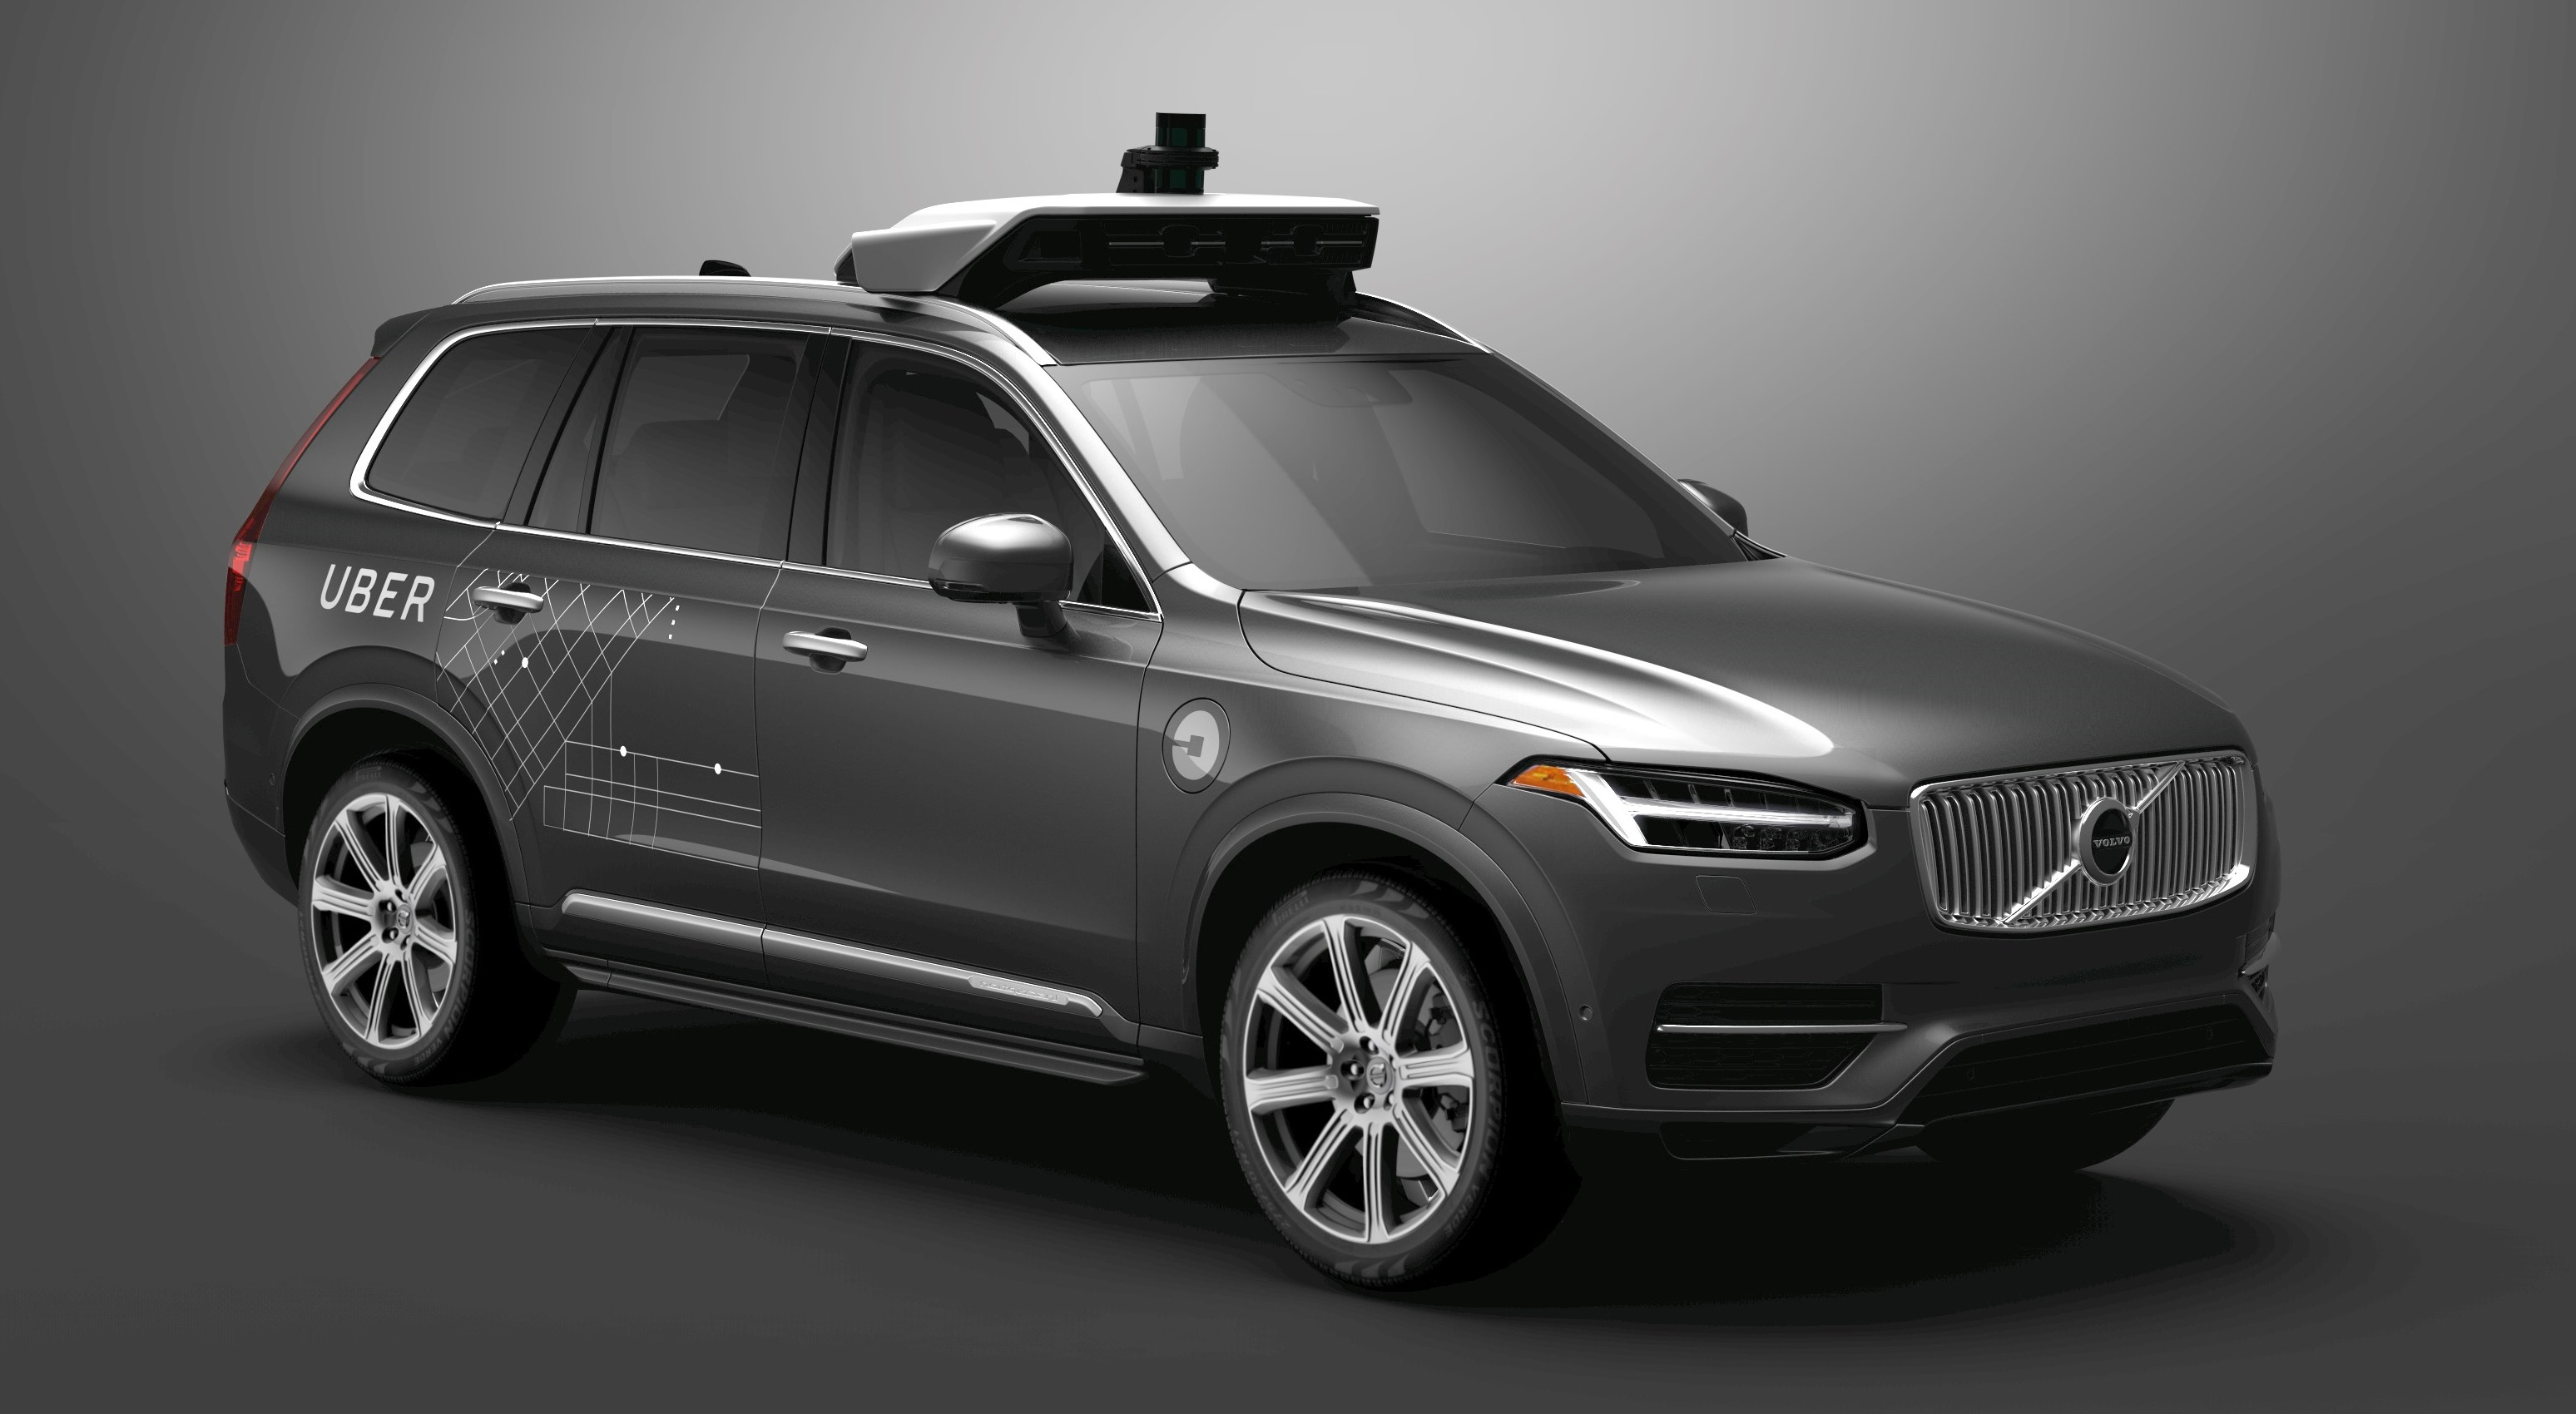
\includegraphics[width=1\linewidth]{materials/chapter_introduction/volvo.jpg}}
\caption{Self-driving Volvo XC90 developed in collaboration with Uber. As of August 2016 pilot project is being launch in Pittsburgh, USA \citep{uberpittsburgh}. Photo reproduced from: \citet{volvo1}}
\label{fig:volvo}
\end{figure} 

\par
Another company that achieved significant successes is Audi with its Piloted Driving project. The company managed to develop a racing car capable of beating a professional driver on a racing track. Nonetheless, Audi is also developing technologies for civil driving \citep{audi1}.

\par


While vehicles on the 3\textsuperscript{rd} level of autonomy are currently only research projects, there are increasingly more commercially available vehicles that have features characteristic for the 2\textsuperscript{nd} level of autonomy. The prime example is Tesla's Autopilot that drives itself on the highway and is able to actively change lanes on a motorway when instructed by the driver \citep{tesla2}. Other examples are the latest premium segment cars by BMW and Mercedes that have features such as lane departure warning, adaptive cruise control or traffic jam assistant \citep{bmw}; \citep{mercedes1}. According to the guidelines by NHTSA, car classified as 2\textsuperscript{nd} level of autonomy must be able to combine at least two of these abilities simultaneously.


\par

Apart from projects run by private companies there are also numerous initiatives supported by public resources. An example of these is the VENTURER Project run by a consortium of academic, public and private  organizations. The people responsible undertaking this will start testing on regular roads in 2017.

\par
Although most of these projects bloomed in the last decade, the idea of autonomous or automated vehicles is considerably older. The first attempts of automating the whole process of driving or only a part of it were made in year 1977 when researchers at Tsukuba Mechanical Engineering Laboratory in Japan built a car that followed white markers and could reach a speed of 20 mph \citep{forrest2007autonomous}.





\paragraph{Views on the future}
\paragraph{}
In the near future we should observe more and more autonomous vehicles appearing on the roads. As mentioned before, fully autonomous traffic is not predicted to happen before the year 2040. The next 30 years should bring significant technological development, along with much needed new legislation and social changes.
\par
It should soon be possible to create a vehicle classified in the 4th level of autonomy. According to \citet{nhtsa1}, a vehicle featuring the 4th level of autonomy should always be able to perform safety-critical driving operations and the driver will not be asked to take over control in any situation. Ford claims to deliver such a vehicle without a driver, steering wheel and pedals by the year 2021 \citep{ford1}.

\par


It is likely that in the midterm future another idea of connected vehicles may become reality. The idea states that vehicles that are close to each other can communicate and therefore increase the safety and add a level of intelligence to their behaviour. Vehicles can also connect to infrastructure and e.g. predict the traffic lights sequence \citep{narla2013evolution} ; \citep{luettel2012autonomous}.

\par
Another prediction is that the development of new legislation can be slower than the development of the technology. Although the fully autonomous car may exist, it might be still required to supervise it from the driver's seat \citep{luettel2012autonomous}. None the less, the UK government claims to be aware of these necessary changes. The report released by UK Department of Transport titled `The Pathway to Driverless Cars Summary report and action plan` \citep{pathwaytodriverless} states that government recognises the benefits of autonomous vehicles and is undertaking actions to aid the development of technologies and law that would allow to bring driverless cars on public roads'. Additionally, the \citet{pathwaytodriverless2} informed that \textsterling 19 million is currently being provided  to allow testing of automated vehicle technology.

\par
Although the majority of the literature focuses on various technical aspects of driverless cars, there are also certain concerns about whether the development is going into the right direction. \citet{mcbride2016ethics} gives Oxford University’s Robotcar as an example and  says that the pursuit of full autonomy does not properly recognize the separation between a human and a machine. The author claims that self-driving vehicles should not be allowed to drive without being deeply connected to the infrastructure, internet and other users.



\par
All in all, in the next years we will observe more development in all aspects of autonomous driving. 
During that time, autonomous cars are likely to be still limited to structured, predictable environments.
We may encounter some challenges mentioned in this section or find new ones that we were not able to predict \citep{luettel2012autonomous}.



%In the next years  Despite the advancements in computer vision, cars may be unable to deal with inconsistent lane marking or unusual, complicated scenarios such as construction site. 



%\par


%not only regular cars but also agriculture. %\citep{luettel2012autonomous}

%\citep{kitti2012we}

%future:
%http://www.forbes.com/sites/eco-nomics/2012/09/25/self-driving-cars-will-take-over-by-2040/#7c83ac1c21f2


\subsection{Implications of autonomous cars revolution}

%advantages and disadvantages...


%\subsubsection{Implications of autonomous cars revolution}
%(including increased demand)
\paragraph{}
Experts around the world argue about the consequences of introducing self-driving cars. The report by UK Department of Transport `The Pathway to Driverless Cars: Summary report and action plan` summarizes some main benefits of having autonomous cars \citep{pathwaytodriverless}. The most important points include a significant reduction of time spent in vehicles and largely improved safety. It is stated that an average driver could save up to 6 working weeks of driving time in a single year. The claim on potential safety improvements is backed by existing evidence from automated vehicles that are already commercially available and feature level 2 autonomy. 
\par
Other important benefits include reduced gas emission and improved congestion. According to the \citet{pathwaytodriverless}, vehicles that are connected into one system would be able to drive in the interest of all traffic participants and therefore greatly optimize traffic. Consequently we should observe a reduction in the Total Kilometers Traveled and increased access to vehicles for everyone \citep{pathwaytodriverless} ; \citep{drivewave}.
\par

On the other hand, it is argued that autonomous vehicles will not be as robust as expected and traffic parameters will, in fact, worsen \citep{sivak2015road}. Additionally, according to Toyota Scientists \citep{toyota1} automated cars may in fact boost fuel consumption as people will be encouraged to travel farther to work. In the example given in \citet{litman2014autonomous}, a family decides to settle further from the city because they can spend time in the car productively rather than controlling the vehicle. In consequence, the benefits of faster and more optimized travel will be counteracted by an overall increase in road demand. Consecutively the traffic parameters may not improve as expected and the amount of VKT will increase \citep{litman2014autonomous}. This concept is also referred to as the Fundamental Law of Traffic Congestion. Any factor aiming at the reduction of traffic can encourage people to travel more. Consequently this will raise overall demand and the traffic will reach its new capacity \citep{duranton2011fundamental}.

\par
Another possible implication is a change in how vehicles are used in general. Concepts such as the `sharing economy` and `collaborative consumption` may result in vehicles being offered as a service rather than being privately owned. The concept of Vehicles-as-a-Service may also eliminate taxi services in the currently known form  \citep{levinson2015climbing}.



%good:
%Autonomous cars: The tension between occupant experience and intersection capacity
%http://www.sciencedirect.com/science/article/pii/S0968090X15000042


%Rely heavily on:
%\citep{litman2014autonomous}

%adittionally:

%http://www.citylab.com/tech/2015/06/these-futuristic-driverless-car-intersections-forgot-about-pedestrians-and-cyclists/394847/


%no taxis probably

%better traffic... faster!



%and:
%The future of travel: How driverless cars could change everything:
%http://edition.cnn.com/2013/05/14/business/bussiness-traveller-futurecast-driverless-car/




%sivak again:
%Influence of Current Nondrivers on the Amount of Travel and
%Trip Patterns with Self-Driving Vehicles







%\paragraph{Maximum Capacity Theorem}
%Traffic has an ability to self organize close to its capacity. This rule called Fundamental Law of Traffic Congestion or Maximum Capacity Theorem states that when stock of available roads rises, the overall driving increases too \citep{duranton2011fundamental}. The theory behind it explains why building new roads or adding new lanes does not necessary yield proportional decrease in congestion.

%Duranton and Turner identified four major sources of additional traffic such as increased commercial traffic, alteration to individual driving behaviour, population growth and diversion from other roads. Raised availability of roads cause an increase in Vehicle Kilometres Travelled (VKT) by commercial vehicles as well as private commuters. Choosing a car as a mean of transport will appear as a more attractive option. 


%This theorem could be put in the context of autonomous vehicles. As mentioned before, introducing autonomous cars to the traffic should result in reduced congestion as travelling would be more optimized. However, according to the Fundamental Law of Traffic Congestion, less traffic on the roads 




%\paragraph{people will cooperate with autonomous cars, }
\par
%including Conflicts, collisions and interactions on the road


\subsection{Main challenges to bring autonomous cars to the roads}
\paragraph{}
This sub-chapter attempts to identify the main challenges that have to be overcame in the following years. Apart from the necessary technological advancements discussed in previous sections, it is also important to focus on other factors such as legislation, safety and public acceptance of autonomous cars. Although these issues were identified as major there are also others that were not covered here.


\paragraph{Law regulations on autonomous driving}

\par
Currently one of the main documents defining the law applicable to autonomous cars is the Vienna Convention on Road Traffic. It states that "every driver shall at all times be able to control his vehicle". This means that as long as this document remains in power, fully autonomous driving will not be possible \citep{vienna1}. However, the UK government has never signed the Conventions that was accepted by multiple countries around the world including a majority of European countries. Therefore, the UK is likely to be in the forefront of the development of autonomous driving as it develops its own legislation \citep{telegraph}.

\par


UK government is aiming to achieve a `light-touch`, non-regulatory approach to introducing new legislation. It is recognised that only a certain level of involvement in the development of technology is necessary in order to achieve the fastest progress.
\par


\par
The \citet{pathwaytodriverless2} document covers wide range of legislation issues associated with autonomous driving. The most important matters include possibly to run tests is real traffic, accounting for other road users and  responsibility in case of an accident. The latter is a commonly discussed issue as it is nor clear whether the driver, the car manufacturer or someone else should be liable for the actions of an autonomous car. 

\par
In USA the statement released by the U.S. Department of Transportation also recognises the significance of autonomous cars underlining the priority of ensuring safety of all traffic participants \citep{nhtsa1}.
\par

%something from usa:
%http://www.nhtsa.gov/About+NHTSA/Press+Releases/U.S.+Department+of+Transportation+Releases+Policy+on+Automated+Vehicle+Development


%SHOULD WE REQUIRE LICENSING TESTS AND GRADUATED LICENSING FOR SELF-DRIVING VEHICLES?
%http://www.umich.edu/~umtriswt/PDF/UMTRI-2015-33.pdf

%A lot more from this The Pathway to Driverless Cars - a detailed review of regulations for automated vehicles technologies

%and this a little bit:
%he Pathway to Driverless Cars Summary report and action plan

%also limitations of computer vision - %\citep{kitti2012we}


\paragraph{Safety}

Safety is one of the biggest concerns tied to autonomous vehicles. Most sources agree that once autonomous cars will be in common use and will be interacting only with each other, we will be observing a creation on an entirely new driving environment; one that is efficient and accidents-free. Nevertheless, before that happens, multiple questions need to be answered: How will the car behave in the situation when it cannot avoid an accident, how will it solve moral dilemmas, the issue of liability for accident  - those are mere examples of such questions \citep{techtimes}. 
 


\par
Before the fully autonomous cars can appear on the roads there is another safety concern regarding human control. It applies to the cars that are not driving entirely on their own and can ask human driver to take control in certain situations. The danger of the handover manoeuvre comes from the fact that once drivers gives control over to AI, his or her reaction time drops dramatically \citep{merat2009drivers}. Recently there was a fatal accident involving Tesla's Autopilot. The exact causes of the accident have not yet been found yet but one of the theories is that the driver was not able to react quickly enough when the car asked him to reclaim control \citep{teslacrash}; \citep{tesla4}. 

\par
Another safety concern applies to emergency situations when the autonomous car has to suddenly decide between trying to save its passengers or a pedestrian. This dilemma touches on ethical issues as the answer is naturally not obvious \citep{qz}. The questions as to whether the cars should kill their own passengers to save a pedestrian is not an easy one to answer and remains one of the most complicated moral dilemmas that have to be addressed before self-driving cars become reality \citep{bonnefon2015autonomous}.

\par

Another possible issue concerns cyber-security. Autonomous vehicles  will be connected to the network and it will be possible for unauthorized individuals to get into the car's operating system and take control over its actions \citep{douma2012criminal}. Another dangerous scenario involves a malware spreading through the car fleet causing damage to the vehicles and putting the drivers’ lives in danger. Proper security measures should be ensured in order to guarantee that such situations will never take place.


%is in no has to choose whether to safe the passengers or pedestrians. 

%Another question of safety concerns the decision that autonomous car 

%http://qz.com/536738/should-driverless-cars-kill-their-own-passengers-to-save-a-pedestrian/





%benefits of heaving a lead car ahead:
%Kountouriotisa, G. K., Merat, N. (2016) Leading to distraction: Driver distraction, lead car, and road
%environment. Accident Analysis and Prevention 89

%hacking cars





\paragraph{Public acceptance of autonomous driving}

\par

The last challenge discussed concerns public acceptance and awareness. The autonomous car revolution can bring very significant changes to the way we travel. To fully enjoy all benefits, the public opinion has to understand the principles of technology and consciously take part in the upcoming changes. This section analyses results of two surveys asking people from various environments on their opinion on autonomous cars.

\par
The first survey was run in year 2014 and included 1500 people from USA, UK and Australia. First findings were that around 60\% of people have heard about the autonomous cars and in general have positive opinion on the subject. When asked about possible improvements that self-driving cars will most likely bring, most participants indicated fewer accidents, reduced severity of crashes, shorter travel time and better fuel economy. Next, people were asked about their main concerns. The most popular answers were legal liability of drivers, data privacy and interactions with non-self-driving-vehicles \citep{schoettle2014survey}.


\par

The second survey involved 5000 people from 109 different countries and asked similar range of questions as the one previously discussed. The results indicated that respondents were mostly concerned with software hacking/misuse, legal issues and safety. It was also found that respondents from more developed countries were less comfortable about data transmission \citep{kyriakidis2015public}.



\subsection{Interactions between human drivers and autonomous vehicles}
\paragraph{}
This section focuses on on-road interactions between traditional and autonomous vehicles. As it is explained later, the matters discussed below lay foundations for the main research questions of this dissertation.

\par
In the next decades driverless cars will be required to successfully cooperate with human drivers. Even when all cars become autonomous, pedestrians, cyclists and other traffic participants must still be able to move around. As discussed in previous section, one of the main public concerns on autonomous vehicles relates to interactions with non-self-driving-vehicles.

\par
Drivewave project conducted by the MIT Senseable City Lab shows how greatly traffic flow can be  improved when there are no human drivers present. The simulation shows how traffic lights can disappear and vehicles could continuously pass though intersection with minimal alterations to velocity \citep{drivewave}. For the traffic with both types of vehicles implementing such a system might not be possible but \citet{dresner2007sharing} suggest a similar reservation system that could manage traffic at intersection consisting both types of vehicles. The idea is that cars approaching the intersection would send information to the intersection manager and receive feedback about action that should be taken.





\par
From the macroscopic point of view, it is not clear whether autonomous cars will increase or decrease the average number of accidents. According to the \citet{excel} most accidents are caused by human error. The main contributory factors are failure to look properly, failure to judge another's person speed or path and driver's carelessness, recklessness or being in a hurry. Driverless cars can potentially be free from these faults.
\par
According to the \citet{pathwaytodriverless} the number of collisions should drop but as aforementioned, according to \citet{sivak2015road}  autonomous cars may be less robust than expected and therefore the number of accident could rise. 


\par
Human drivers have certain expectations towards other drivers. Things like eye-contact are often important for successful communication. That kind of interaction will be absent in encounters with autonomous vehicles. Moreover, human drivers often possess skills and experience that may not be easy to quantify and program into a machine. Therefore, driverless cars can, in fact, perform worse in certain situations and as a result, during the transition period the amount of accidents might in fact increase \citep{sivak2015road}.




%\textbf{Data Shows Google’s Robot Cars Are Smoother, Safer Drivers Than You or I:}
%https://www.technologyreview.com/s/520746/data-shows-googles-robot-cars-are-smoother-safer-drivers-than-you-or-i/


%also

%Replacing the Stop Sign: Unmanaged Intersection Control for Autonomous Vehicles



%\par
%https://www.media.volvocars.com/global/en-gb/media/pressreleases/158276/volvo-cars-presents-a-unique-system-solution-for-integrating-self-driving-cars-into-real-traffic


%\par

%\paragraph{conflicts...}








\subsection{Defining the research scope}

\paragraph{}
This section describes the primary research question addressed in the dissertation. It explains motivation for the study and how it arose from the gap identified in the current state of knowledge. Furthermore, it lists all aims and objectives covered within the scope of the project and later supports their relevance with literature discussed in previous sections.


\par



As it was shown, the interest in autonomous vehicles is enormous. Many corporations and governments are channelling very significant amounts of money to various projects associated with autonomous driving. Every involved organization whose aim is to maximise profits is trying to be at the forefront of this upcoming revolution. The amount of research being done in various aspects of this new field of science is likewise immensely vast. 
\par
The majority of attention is given to the development of technology that would allow to construct vehicles with higher level of autonomy. Next area of interest focuses on possible implications of the revolution and other things such as legislation, psychological dilemmas and public acceptance that has to go along with the technological development. There is however, little study on how the traffic itself will change during the upcoming years of the transition period. Letting autonomous cars drive among traditional ones will bring far-reaching consequences. The main principles of the traffic, as we know it, will have to be redefined to ensure that we experience all of the possible benefits of these changes. 
\par
\textbf{On the basis of the gap identified in the research, this dissertation attempts to develop a broad understanding of how traditional and autonomous vehicles will interact with each other and what will be the consequences of these interactions on a micro and macro scale.}

%*****lovely above


%\par

%It is believed that in order to achieve the most benefits from autonomous driving the algorithms governing the self-driving cars have to be optimized for efficient and safe interactions with traditional vehicles. The study focuses on understanding of these interactions. 

\par 
Further paragraphs describe the main aims and objectives of the project. Aims were distinguished from the objectives as being more abstract and relating rather to contribution while objectives are more real and define specific methods used in the project.



%reflect on original Eddie's idea

%eddie original idea was that :
%-autonomous cars will be very expensive
%-used as a service
%-long transition period



%\paragraph{Aims} - later delete (contribution)
\par
%past tense but talking about future
The primary aim of the research was to predict the impact of autonomous vehicles on the traffic. Results obtained were analysed from the point of view of macroscopic traffic parameters such as average velocity, vehicle density and congestion. The focus of the research was congested, city traffic rather than motorways.

\par

The secondary aim was to inspect particular interactions from the point of view of traffic participants. It was investigated how interactions between two humans compare to interactions between two different types of vehicles.  

%3rd aim? ..or more motivation??
%- jak powinny sie zachowywac auta autonomiczne aby poprawic poprawic parametru ruchu ulicznego
% to samo zeby mniejszyc liczbe kolizji
%- te badanie moga dac wiecej swiatla na jakiego typu interakcje mozemy sie spodziewac 

\par

The main objective of the project was to conduct the experiment that would be a simplified simulation of traffic and would involve human drivers and autonomous cars. The experiment should allow for simultaneous inputs from multiple traffic participants. It would consist of a few different scenario that would involve different proportions of human drivers and self-driving cars. 

\par

The secondary objective was to engineer the software that allowed to conduct the experiment. It had to meet all requirement of the experiment and be able to accommodate for altering number of participants. The main part of the software was a network-based, multi player traffic simulation. Each person participating in the experiment controlled one vehicle and made decisions by observing other traffic participants. By looking into how cars interact with each other it should be possible to extract the impact of self-driving vehicles on the traffic.


\par

In order conduct the study a simplified model of autonomous car had to be created. It is important to note that the development of such a model derived from the needs of the primary research and is not a topic of interest itself. Once the right model was established it remained constant through the whole experiment. The algorithm governing the model was derived from well established principles of common car-following models.


\par

Last major objective was to create a realistically behaving model of car dynamics that would respond to participant's commands according to his or her expectations. 



\par
%justify why the experimn was even done

The main aim of the project was to look into interactions between autonomous and human-driven vehicles. The main method that was used to achieve this was to create a simulation of traffic with both types of traffic participants. By reviewing the literature it was found that there are numerous car-following models that could be used as a model of human driver \citep{rothery1992car}; \citep{treiber2013traffic}. However, no matter how good were these models, they could only work as an approximation of how humans would actually control the cars. It was decided that differences between any of the reviewed car-following algorithms and the unpredictability of real human control are so significant that the study should rely on the experiment involving multiple human participants simultaneously controlling cars in interconnected simulation.
 \par
The decision to create such simulation was a key factor that gave shape to the whole project and accounted for the majority of the effort. Out of all work conducted through the project designing and implementing software that would allow to successfully conduct the experiment was the most absorbing and time consuming part.



%The main aim of the research is to try to predict what will happen when autonomous cars are introduced to the traditional traffic. Results obtained will be evaluated from two different perspectives. Firstly we will analyse traffic parameters such as velocities, densities and congestion to inspect how the traffic changes from macroscopic point of view. Secondly we will focus on particular interaction from the point of view of traffic participants. It will be investigated how interactions between two humans compare to interactions between two different types of vehicles. 



%The main aim of the research is to determine in which way introducing autonomous cars will affect the traffic. 

% the impact of introducing autonomous cars to the traffic


%trying to predict what will happen when autonomous cars are introduced to traditional traffic. 









%The secondary aim is trying to find guideline for autonomous cars that could be useful in the development of the technology





%each other and how 

% reacted differently when autonomous vehicle was encountered.






%nice paragraph:
%It is believed that in order to achieve the most benefits from autonomous driving the algorithms governing the self-driving cars have to be optimized for efficient and safe interactions with traditional vehicles. The study focuses on understanding of these interactions. 

\paragraph{Reflection upon original project scope}

The original scope of the project included also in-robotico implementation that would be using remotely controlled "slot-cars" to simulate traffic. It was believed that physical model would have features that could not be accounted for or predicted in computer simulation. It was estimated for around 50\% of implementation effort. However, in the final version of the project the physical model was not implemented. After the project went into development the advantages of creating a physical model appeared less and less attractive. Especially compared to the cost of implementation. Original idea assumed using digital slot-car set with cars and track, as well as computer vision to track vehicles on the track and live video streaming to multiple computers. After more careful consideration the benefits of implementing above described would be very minor or none. In addition to this, implementing the computer simulation consumed more time that estimated. 

It has to be admitted that scope was significantly reduced in terms of implementation. It did not, however, have much impact on the quality of the research and conclusions. One would even venture to say that project should only consist of computer simulation even if more time and resources were allowed for project execution. 




\subsection{The experiment}

\paragraph{}

This section discusses the initial design of the experiment. At the start of the software development the exact way in which the experiment will be conducted was not yet known. More and more details on the experiment were being established as the development of the software was progressing. Described below is the level of knowledge on the experiment that was used as the initial guidelines for the development of software.

\par

%First, a general description is given. 


%The description of the experiment given in this chapter 




%********************START HERE **************



%cool above

%\paragraph{Initial description and requirements}

%now all about the experiment itself:
%\par

%The following section describes the level of knowledge about the experiment before the start of implementation.



%At the initial stage of the project the details of the experiment were not yet established. One one the requirement of the software was to account for flexibility required by the experiment..



The experiment was arguably the most important part of the project. All work done before was aimed at successful conductance of the experiment and all work done after was based on the data collected during the experiment. 



\par

The experiment was planned to involve ten to twenty people. They would be asked to control one of the vehicles in the simulation. Each of them would sit in front of a computer where they could use the keyboard and observe the screen. On the screen they would see a simplified top-down view of their own vehicle and it's surrounding. The field of view around each car would be limited to a certain radius around the car to simulate what can be seen from the inside of the vehicle in real life. (maybe figure here alread..?)

\par

The main experiment was planned to consist of a number of different scenarios. Each scenario would be using different shape of the map and would have different number of human-driven and autonomous vehicles. It should be possible to generate maps by giving only the necessary amount of information about the map's shape. Before each scenario it should be possible to set currently required number of human participant and autonomous cars. Flexibility of these parameters should allow to accommodate for unknown number of people that will show up for the experiment.


\par


Participants would control the vehicles using arrow keys on the keyboard. The vehicle should respond immediately and in a predictable way. Participants should be able to control acceleration of the car and make discrete choices on the turning direction. Additionally participants should be informed about their current speed.  
\par

The refresh rate of the simulation should not have impact on the results of the simulation. Participants should be able to perceive the environment without any noticeable delay. It should be possible to change the rate if necessary. The initial value of the frame rate was 25 frames-per-second and was inspired by traditional frame rate in films. 
At each iteration the state of the whole simulation should be stored for future analysis. 

\par
The model of the autonomous car should be relatively simple. The algorithm behind the model should allow to dynamical move around the map on predefined path and successfully avoid collisions with all other participants. The level of knowledge of the autonomous car could be higher than experiment participants'. This is supported by the view that autonomous cars are likely to have access to knowledge coming from centralized sources or intelligent infrastructure.

\par
In order to encourage people to come to the experiment a monetary reward and catering should be available. There should be a strict control on what information is being revealed to the participants before and during the experiment. The main part of the experiment should be preceded by short questionnaire describing driver's profile.

\par




%%%%%%%%%%%%%%%%%%%





\subsection{Roadmap}

\paragraph{}

The implementation of the project consisted of three main parts. First one was software development which accounted for around 50\% of all efforts. Next chapter is dedicated entirely to this topic. It is divided into most significant components that include the reasoning behind the choice of the development environment, design of the simulation server, design of the client's application, design of autonomous car's dynamics and the description of network solution used in the project. 

\par

Next chapter is dedicated to all aspect of the experiment. First part defines exactly what the experiment consisted of. Next one describes client's interface design and reasoning behind it. Third one describes the dynamics of the car controlled by participant and compares it with autonomous model. Last section reports about the experiment execution including the survey and minutes.

\par

Next chapter talks about the results of the experiment. It is divided into two main parts: observations and hypotheses. Part on observations relates to patterns that were identifiable in the collected data. Part on hypotheses suggests three assumptions and attempts to verify their genuineness.


\par

Last chapter summarizes the project and draws conclusions. Additionally, it also suggests ideas for future work.

%The chapter on research methodology also describes how communication between machines was established and the algorithm behind autonomous vehicles. Although these two aspects were integral parts of the software it was decided to write about them separately due to the significance and universality of communication solution and autonomous car algorithm. 
%Most of decisions made throughout the development stage were aimed for successful experiment execution. The design of the experiment is described at the of Research Methodology chapter. The description of how the experiment was eventually conducted is placed at the begging of Finding and results chapter.


%The Research Methodology chapter is preceded with in-depth chapter describing literature relevant to the project. The data obtained during the experiment was described in Findings and Results chapter. This chapter also talks about different ways in which data was analysed. The last two closing chapters discuss the results of the experiment, attempt to draw conclusions and generalize findings in wider context. 

%%%%%%%%%%%%%%%%%%%%%%%%%%%%%%%%%%%%%%%%%%%%%%%%%%%%%%%%%%%%%%%%%%%%%%%%%%%%%%%%%%%%%%%%%%%%%%%%%%%



\newpage
\section{Software Engineering and Model Development}
\paragraph{}
Creating software that allowed to successfully conduct the experiment was the longest and most absorbing part of the project. All decisions starting from the choice of programming environment, through deciding on the structure of the software to ensuring simulation reliability were dictated by the requirements of the experiment. From the point of view of software implementation the experiment required at least two applications running on multiple machines that would be communicating with each other over the network in real-time.

\par

This chapter outlines all software developed prior to the experiment. First section is dedicated to the choice of the development environment. Next one describes two main components of software: simulation server application and client's application. The third one characterizes models of car dynamics used in the simulation and reasoning behind choosing them. The last section explains the network solution used in the experiment and the path the led towards it.

\par

%***more planned to be added here...


%The aim of the softwa

%Scalability - although traffic was represented in a very simplified way, the goal was to identify the most important factors influencing 

%Reliability - software should be tested for different circumstances. 

%To ensure validity of the results some basic principles were followed throughout the whole process:


%//say about the aims of the software. what makes good software good? maybe look here:
%https://medium.com/@mbostock/what-makes-software-good-943557f8a488#.djbqo2es9



%//write more intro to software



%say how this was not important o avoid cheating as described by Arthur earlier



%Justify all major design decisions

%Justify all major design decisions. Plenty of them!
%All the actions undertaken to ensure most meaningful results


\subsection{Environment choice}
\paragraph{}

Choosing the right environment to develop software was a key decision that had crucial impact on all components of the project. After a process of careful consideration it was decided to use MATLAB as a sole development environment for all parts of the project. 
\par
The initial Project Proposal written by project supervisor, Eddie Wilson suggested using SUMO package as a core of the simulation. 
\par

%\paragraph{Traffic modelling software, (SUMO)}

SUMO stands for Simulation of Urban MObility. It is an open source framework used for traffic simulation \citep{krajzewicz2002sumo}. SUMO was first introduced in 2002 and since then it became a popular tool for scientist as well as people involved in practical traffic planning tasks. 
\par
SUMO is a purely microscopic simulation which means every traffic participant is modelled separately. The framework is designed to simulate large cities that contain thousands of roads and more than one million of vehicles.
\par
The core of the SUMO package is a logical representation of road layout. Segments of roads separated by junctions are described as nodes and edges. Edges consist of directed lanes. Vehicle's position is described in terms of edge and lane number and distance from origin node. At every step of the simulation interactions between individual simulation entities are computed and all parameters updated 
\citep{krajzewicz2002sumo}.
\par

It was assumed that a small part of SUMO capabilities would be utilized in combinations with additional software written for the purpose of this project. SUMO features  Traffic Control Interface (TraCI) \citep{sumo2} that gives access to the running simulation. The parameters of the simulation like car's location could be potentially retrieved and manipulated in real-time. The additional software would be responsible for network data exchange, visualizing car's surrounding and capturing inputs from experiment participants. Most likely the programming language used for this part would be C++. 
\par
On the other hand, SUMO was intended for much larger simulations than the one planned. Vast majority of available features would not be used and could rather be a source of potential issues. 


%%%%%%%%%%%%%%%%%%%%%%%%%%


\par


A competing idea was to create a tailored application that would be inspired by the structure of SUMO but would be written from scratch. It would be implemented using C++ or MATLAB environment. The main benefit of this approach would be full control of the software behaviour. The main drawback would be rewriting algorithms and structure that already existed inside SUMO. In terms of subjective software preference MATLAB was considered most familiar and least error prone.  

\par

Another key question that had large impact on the decision was how to establish reliable communication between machines. It was found that MATLAB supports at least three possible ways of communication that could be used in the project including User Datagram Protocol (UDP), Transmission Control Protocol (TCPIP) and Robot Operating System. Out of these three ROS was considered as a primary network solution.

\par
Although ROS is a framework designed for the development of robots, it also provides structured communication layer \citep{quigley2009ros}. Applying ROS would allow to reliably send data either as a point-to-point communication or as broadcasting.

\par
 This was the main reason why MATLAB was eventually chose for this project.
Details of the implementation of network communication are described in the chapter \textit{Communication between machines}.




\subsection{Software architecture}
%***(present tense here..?)

The software in the project consists of three  main parts. The most important one is simulation server application. It is responsible for all data processing that is essential for the simulation. The second piece of software is simulation client application. Each participant used an identical copy of simulation client application to receive information about car's surroundings and send acceleration and direction orders to the server. Last part of the software is the communication agent which was responsible for aggregating information from all clients and sending it to the server. Its existence was dictated by the requirements of network solution described in further chapters. server, agent and all clients' applications were running on separate machines.
\par
Central part of the simulation was the main loop that was executing at fixed rate of 16 Hz. All machines used in the experiment were synchronized according to server's clock. This simplified sequence of events across all applications is described in Table~\ref{table:simple_events}.

\par

%This chapter describes the most important aspects of the implementation of Simulation Server Application followed by the description of Client's Application



% Please add the following required packages to your document preamble:
% \usepackage[table,xcdraw]{xcolor}
% If you use beamer only pass "xcolor=table" option, i.e. \documentclass[xcolor=table]{beamer}
%\begin{tabular}{|p{4.3cm}|p{4.3cm}|p{4.3cm}|}
%\begin{tabularx}{\linewidth}{ r X }
%    right-aligned foo & long long line of blah blah that will wrap when the table fills the column width\\
%\end{tabularx}

%\begin{tabular}{|l|l|l|}

\begin{table}[]
\centering
\begin{tabular}{|m{4.4cm}|m{4.4cm}|m{4.4cm}|}
\hline
\multicolumn{1}{|c|}{\textbf{Simulation Server Application}}     & \multicolumn{1}{c|}{\textbf{Communication Agent}}  & \multicolumn{1}{c|}{\textbf{Client(s) Application}} \\ \hline
Starting ROS Core and opening UDP ports for Clients and Agent    & Connecting to ROS node and opening UDP ports       & Connecting to ROS node and opening UDP ports        \\ \hline
Setting up simulation parameters                                 & Listening to instructions from Server...           & Listening to instructions from Server...            \\ \hline
Sending configuration messages to Clients                       & Listening to instructions from Server...           & Receiving configuration messages from Server        \\ \hline
Sending start order to Clients and Agents. Starting main loop                       & Starting main loop                                 & Starting main loop                                  \\ \hline
\multicolumn{3}{|c|}{\textbf{Main loop}}                                                                                                                                    \\ \hline
Sending individual messages to each Client                       & Sending combined orders from all clients to Server & Sending order to Agent                              \\ \hline
Receiving combined orders from Agent                             & Trying to receive from every client one by one     & Receiving my location and vehicles' around me       \\ \hline
Performing all calculations for clients, map and autonomous cars & Combining orders from all client to one message    & Performing calculation and drawing map in viewport  \\ \hline
\textit{Waiting for next loop iteration}                         & \textit{Waiting for next loop iteration}           & \textit{Waiting for next loop iteration}            \\ \hline
\end{tabular}
\caption{Simplified order of events across all applications. The order of the events in Agent resulted in one frame delay between giving order by Client and receiving it by Server.}
\label{table:simple_events}
\end{table}






\subsubsection{Simulation server application design}
\paragraph{}

Simulation Server Application was at the heart of the simulation. It was responsible for all essential computation, managing communication between other entities and executing code at a constant rate.
\par
This section starts with an overview of class structure within the application followed by a description of the sequence of events happening in main simulation loop. It then talks about the server side interface and the structure of messages send between other entities.

\par

The design of server side application consisted of following classes (appendix: class diagram):

\begin{itemize}
\item Simulation - Only one object of this essential class existed thoughout the entire simulation. The most important methods were accountable for establishing communication, importing parameters and running the main simulation loop.
\item Map - Single Map object was created by Simulation. Among other things it contained all information regarding road layout, references to all vehicles, relations between them and future predictions. 
\item Car - Base class was intended to derive other classes from it. It contained features common for both types of vehicles such as velocity and distance calculations and Gipps model.
\item Car human driven - Derived from the Car class. It contained additional attributes specific to the human-driver but only basic methods as most of essential computation was happening within Map class.
\item Car autonomous - The Intelligent Driver Model and decision making algorithm were encapsulated within this class. It was receiving limited information about car surrounding from Map object.
\item Participant - Additional class created to separate orders received from participants from car's logic.
\end{itemize}


The sequence of events in the main loop of the simulation was as shown in Table~\ref{table:order_server}. While Simulation object hold supervision role over whole process, the Map object was responsible for the majority of tasks. Once Simulation received information from communication agent and passed it to Map, most commands were called on the basis of Simulation object asking Map object to do certain things and return some values which were then passed to e.g. Autonomous Car. An additional feature of Map class was an ability to create large raster images of the whole track. These images were later used by Client Application.


\begin{table}[]
\centering
\begin{tabular}{|l|p{2cm}|p{11cm}|}
\hline
\textbf{} & \multicolumn{1}{c|}{\textbf{Class}} & \multicolumn{1}{c|}{\textbf{Event}}                                                                    \\ \hline
1         & Simulation                          & Sending each Client its location and orientation together with information about surrounding vehicles. \\ \hline
2         & Simulation                          & Receiving message from Agent containing movement orders from all Clients                                \\ \hline
3         & Simulation                          & Extracting orders from each individual Client                                                          \\ \hline
4         & Simulation                          & Passing updated cars' movement orders to Map object                                                    \\ \hline
5         & Map                                 & Predicting position of all cars up to 3 seconds ahead based on current velocity and movement order     \\ \hline
6         & Map                                 & Calculating collisions for current time and predictions made in last step                              \\ \hline
7         & Map                                 & For each autonomous vehicle finding potential collisions with other vehicles                           \\ \hline
8         & Autonomous Car                      & Making decision on desired acceleration on the basis of information supplied by Map                    \\ \hline
9         & Human Car                    
& Calculating target acceleration on the basis of received acceleration order                            \\ \hline
10        & Car                                 & Calculating traveled distance using 4th order Runge Kutta equations                                    \\ \hline
11        & Map                                 & For each vehicle calculating new position and edge on map topological structure                     \\ \hline
12        & Map                                 & For each vehicle calculating new Cartesian coordinates and orientation                                 \\ \hline
13        & Map                                 & Preparing individual messages for each Client                                                          \\ \hline
14        & Map                                 & Drawing all vehicles on the map in Simulation Server GUI                                               \\ \hline
15        & Simulation                          & Saving simulation state at current step.                                                               \\ \hline
16        & Simulation                          & Waiting for next loop iteration                                                                        \\ \hline
\end{tabular}
\caption{Order of events in main simulation loop in Simulation Server.}
\label{table:order_server}
\end{table}


\paragraph{Server's graphical interface}


In order to simplify the simulation control and supervise simulation status a simple server-side graphical interface was created. It's two main functions were displaying position of each car on the map and setting up each scenario configuration. Figure~\ref{fig:master_gui_small} shows a top-down view of the whole map available in the GUI. The interface capabilities allowed to start the ROS node, open the UDP ports, choose number of cars of each type, choose a map, send configuration messages to other parties and start or stop the simulation. 

\begin{figure}[!] % Example image
\center{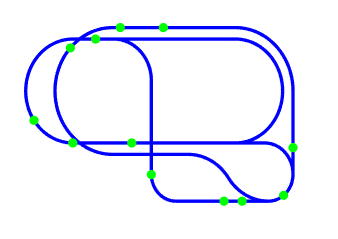
\includegraphics[width=0.7\linewidth]{materials/research_methodology/master_gui_small.png}}
\caption{Visualization of current simulation status available via Simulation Server GUI. This example shows third map with 14 autonomous cars.}
\label{fig:master_gui_small}
\end{figure} 



\paragraph{Centralized control}


Running synchronized processes on multiple machines was a significant challenge and a source of potential issues. While the details of network communication are described later, additional, high-level measures were taken to simplify simulation management. The messages send between machines were always in the form of formatted strings. Throughout entire simulation clients and agent were always listening to messages broadcasted from the server. This allowed to manage the simulation from Server without any additional configuration on each single computer. There were two basic types of messages: configuration messages starting with letter 'c' and current simulation messages starting with letter 'm'.
Configuration messages were usually sent outside of the main loop and contained information about next simulation session such as map size, map name, initial location of vehicle. These messages were also used to start or stop the simulation. To identify the message the first letter was followed by a 3-digit code that was understandable for both parties. An example of a map size configuration message is shown below.

\begin{equation}
c \quad 108 \quad 0 \quad 360 \quad 0 \quad 260
\end{equation}

First number 108 meant that map size is being sent. Rest of the message was then interpreted as x and y dimensions of the current map.
Current simulation messages were often more complicated. Below is an example of message send from master to client in running simulation. 
 
\begin{equation}
m \quad 124.56 \quad 189.70 \quad 43.1 \quad 10.8 \quad 1 \quad 2 \quad 141.5 \quad 164.9  \quad 56.2 \quad 135.5 \quad 150.4  \quad 66.8
\end{equation}

First 3 numbers stood for car's location and orientation. Next two numbers indicated current speed to be displayed on speedometer and binary collision status (participants were informed when collision occurred). Yet another number indicated how many other cars are in the surrounding. All numbers that followed described those cars' locations and orientations. That data was then used by the client to draw a map and all vehicles in the view field. If the message received was distorted or incomplete and therefore different from what was expected, it was rejected and values from previous iteration were used.






\subsubsection{Client application design}
\paragraph{}

Identical copy of Client Application was deployed on  each computer used by experiment participants. Main tasks of Client Application included receiving location and orientation, sending acceleration and turn order, displaying part of the map to the participant and harvesting inputs from the keyboard. Its design consisted of following classes (appendix: class diagram):

\begin{itemize}
\item Simulation client - Main class. Responsible for communication with Server and Agent and management of whole simulation from client's side. 
\item Map client - The most important class. Responsible for such essential tasks as displaying the map and cars in GUI
\item Car client - Relatively simple class containing some essential parameters of the car. 
\item Participant - Identical to the class used by Simulation Server Application. It contained some attributes that should be separated from Car client object.
\end{itemize}


The sequence of events happening at each loop iteration is shown in Table~\ref{table:clients_events}. As it can be seen, it was considerably simpler than Server Application. 

\begin{table}[!]
\centering
\begin{tabular}{|l|l|l|}
\hline
\multicolumn{1}{|c|}{\textbf{}} & \multicolumn{1}{c|}{\textbf{Class}} & \multicolumn{1}{c|}{\textbf{Event}}              \\ \hline
1                               & Simulation client                   & Sending acceleration and turn orders to Agent    \\ \hline
2                               & Simulation client                   & Receiving locations and orientations from Server \\ \hline
3                               & Simulation client                   & Displaying speed and collision status on GUI     \\ \hline
4                               & Map client                          & Cropping and rotating map image                  \\ \hline
5                               & Map client                          & Displaying cropped map image in viewport         \\ \hline
6                               & Map client                          & Overlying cars on the map                        \\ \hline
7                               & Simulation client                   & Waiting for next loop iteration                  \\ \hline
\end{tabular}
\caption{Order of events in the main simulation loop in Simulation Client.}
\label{table:clients_events}
\end{table}


\paragraph{Displaying map in the view port}

Displaying car's surrounding was one of the main challenges in the implementation of client's application. As discussed earlier, the experiment design required showing a top-down view of a rectangular area around the car together with the car itself and all other cars contained in the view port. From the beginning of the design process, two, radically different approaches to achieve this goal were analysed. First idea, was to calculate coordinates of each point required to render scene and display the results using one of MATLAB plot functions. This approach would allow for full scalability and could potentially result in appealing map image without visible pixels. On the other hand, the amount of calculations could be much greater, as not only cars and road were to be computed but also multiple stationary objects around the road that were supposed to improve the felling of speed (such as trees or houses). 
The second idea for the representation of view port was to crop and rotate part of the map stored as a large, raster image. The  map image was supposed to be 2 to 5 thousand pixels wide and at each loop iteration a part of it would be cropped and rotated according to current car's location and orientation and then showed on client's GUI. Subsequently, all vehicles would be plotted over the image. The main advantage of this approach would be a possibility to use complex map image which could be rich in diverse, colourful features. The main drawback would be less attractive, pixelated image as the resolution would be limited. 
After initial trials with each approach, second one was chosen for the implementation. As it quickly turned out, the main challenge was limited computational power of machines used in experiment. One iteration could not last longer than 0.0625 s and preparing map image was only one of the tasks that had to be executed (the frame rate was limited from 20 FPS in later stages of implementation due to Server Application performance reasons). To overcome this problem, a custom function to crop and rotate was written. It was used instead of MATLAB methods \textit{imcrop} and \textit{imrotate}. The backbone of this function was written by project supervisor, Eddie Wilson. It was later adapted according to the requirement of the GUI. 
Once the cropped image was displayed on the GUI, vehicles were plotted over it using MATLAB \textit{patch} function. The overall performance of this solution was sufficient for the needs of the experiment. It allowed to display images 480 pixels wide and tall with plenty of room left for remaining tasks.




%\paragraph{Harvesting inputs form participants} - maybe actually put it in car control



%Client application was used to communicate with experiment participant

%Client application was responsible for receiving 

%Client application was responsible for two-way communication with experiment participant. Each participant used exact same copy of client application. 


%***DRAFT***



%It was tried to mimic the way cars are controlled in popular computer racing games such as Need For Speed\textsuperscript{TM}. 

%The behaviour of cars controlled by humans 


%here combined technical solutions 

%General description Simplifications and yet still accounting for most important parts of the car model

\subsection{Modelling car dynamics}
\paragraph{}
One of the requirement of the experiment was to create two models of cars that were meant for two different purposes. One of them was a model of an autonomous car that makes its own decisions and the other one was a model a car that can be controlled by the experiment participant. 

\par
This section firstly gives examples of the most significant car-following models and describes how two of them were used to create models for this simulation. Section is summarized by a succinct comparison of these two models.



\subsubsection{Car following models}
\paragraph{}
Car following models are the most fundamental part of any microscopic traffic modelling \citep{treiber2013traffic}. They describe car's behaviour on the basis of the state of the car in front. Nevertheless, a complete car following model is also able to describe behaviour in free flow or when there is a stationary obstacle in front of it. There are various models dedicated to different kinds of research. One of the simplest examples is the Optimal Velocity Model which calculates the acceleration on the basis of the intervehicle distance. It is however, not very robust and the results are unrealistic. 
\par
More realistic models are based on various driving strategies. The prime example is the Gipps' model \citep{treiber2013traffic}; \citep{rothery1992car}. It is able to vary its acceleration depending on the time gap to the vehicle in front. It's braking manoeuvres always feature constant deceleration and there is no distinction between comfortable and emergency braking. Gipps' model is considered the simplest accident-free model. Within a certain range of parameters, it produces considerably realistic results.
\par
Although the Gipps' model is often used in traffic simulations, it is not fully versatile. The simplest complete and accident-free car following model is Intelligent Driver Model. It is capable of  dealing with virtually any kind of situation. Its acceleration depends on the distance to the car in front, that car's velocity, own velocity and few static parameters. What is more, IDM features Intelligent Braking Strategy. In typical traffic situations its deceleration is limited to some comfortable value. However, during an emergency situation, if something suddenly appears in front of it, the deceleration will rise to minimum value that is necessary to prevent collision \citep{treiber2013traffic}.



\subsubsection{Autonomous car model}


Creating an adequate self-driving model was one of the key tasks that had very significant impact on the experiment. The requirements of the experiment stated that autonomous cars should be able to travel among traditional vehicles, avoid collisions and follow default route. In order to ensure validity of the results the model should aim to preserve the most essential features of real autonomous vehicles. The challenge was to identify these features and implement them to the possible extent. 

\paragraph{Deriving model from IDM}%Intelligent Driver Model
From the point of view of other traffic participants it would be expected that autonomous car's behaviour was familiar and predictable to some extent \citep{sivak2015road}. In order to ensure such performance in this simulation, the model governing the autonomous car was based on Intelligent Driver Model which is briefly introduced in previous section. The model is described with the following formulas:

%one of the most popular car-following models often utilized in traffic simulations \citep{treiber2013traffic}. 


\begin{equation}
\dot{v}=a\left[1-\left(\frac{v}{v_0}\right)^{\delta}-\left(\frac{s^{*}\left ( v,\Delta v \right )}{s}\right)^{2}\right]
\end{equation}

\begin{equation}
s^{*}\left ( v,\Delta v \right )=s_0+max\left ( 0,vT+\frac{v\Delta v}{2 \sqrt{ab}} \right )
\end{equation}
Where $a$ is maximum acceleration, $v$ is current velocity, $v_0$ is desired velocity if there are no cars ahead, $\delta$ is acceleration exponent (the grater the value, the later the reduction of acceleration when approaching  the desired velocity), $s$ is current distance to the car ahead and  $s^{*}$ is desired distance.
In the second formula $s_0$ is minimum gap, $T$ is minimum time gap and $b$ is comfortable deceleration. The values of these parameters were taken from \citet{sivak2015road} as typical values for city traffic and altered according to the specificity of this simulation (Table~\ref{table:idm}).


\begin{table}[!]
\centering
\begin{tabular}{|p{7cm}|p{3cm}|}
\hline
\textbf{Parameter}          & \textbf{Value} \\ \hline
Desired velocity $v$          & $10\:\nicefrac{m}{s}$         \\ \hline
Time gap $T$                  & $0.8\:s$          \\ \hline
Minimum gap $s_0$            & $7\:m$            \\ \hline
Acceleration exponent $\delta$ & $4$              \\ \hline
Acceleration $a$              & $5\:\nicefrac{m}{s^2}$         \\ \hline
Comfortable deceleration $b$  & $7\:\nicefrac{m}{s^2}$         \\ \hline
\end{tabular}
\caption{My caption}
\label{table:idm}
\end{table}



\paragraph{Accounting for traffic coming from different directions} For the purpose of the simulation IDM had to be expanded beyond simple car following. Just as a real autonomous car would do, the model used here observes other traffic participants. For every car in the radius of 60 meters it detects it's current velocity and estimates position from now to 3 seconds ahead. 
If collision is anticipated, certain parameters of IDM are overwritten. A simplified algorithm governing this behaviour is shown on Figure~\ref{fig:idm_upgrade}. It allowed for smooth, predictable behaviour in almost all situations. 


\begin{figure}[!] % Example image
\center{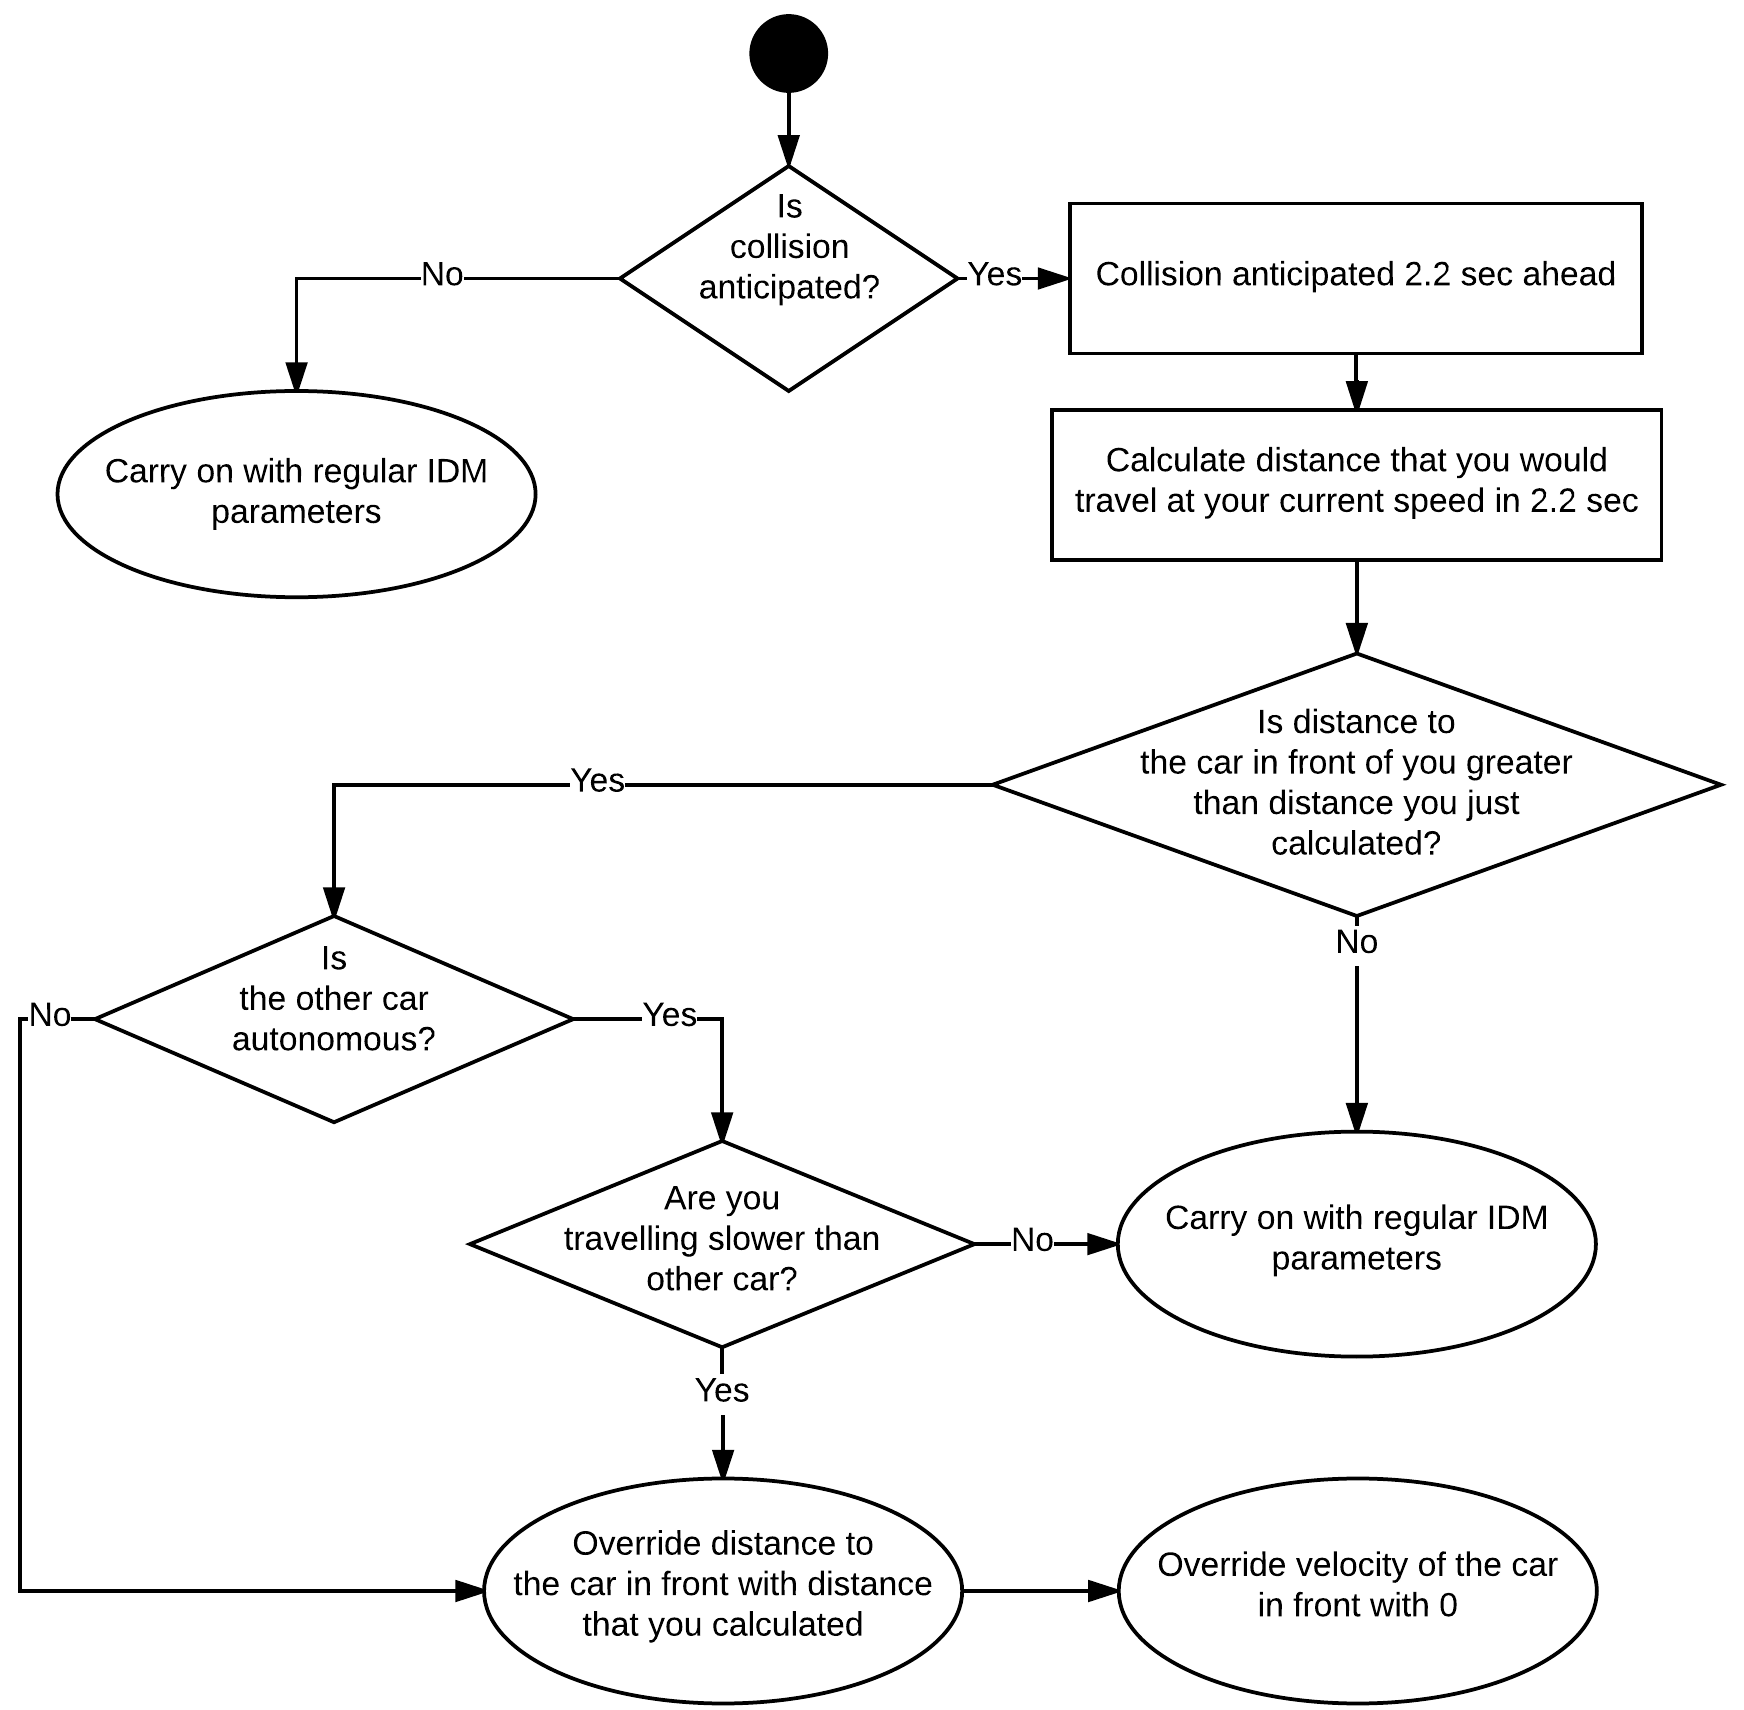
\includegraphics[width=1\linewidth]{materials/research_methodology/idm_upgrade.png}}
\caption{Algorithm governing the behaviour of autonomous car. It was executed for each car at every time step of the simulation. It allowed for very smooth interactions if another autonomous car was encountered and very cautious ones with human drivers.}
\label{fig:idm_upgrade}
\end{figure} 


\subsubsection{Human car control}

The way in which cars were controlled had significant impact on the experiment results. From participant's point of view car's behaviour should be predictable and similar to how real car behaves. The challenge was to achieve this kind of performance using only discreet inputs from keyboard. Graphical interface used by participants allowed to capture multiple keys pressed simultaneously, however resulting acceleration order had to always be one of the following: speed up, slow down, coast or brake. After analysing relevant literature it was decided that car's behaviour should be similar to one of the cars following models \citep{treiber2013traffic}. From The Gipps' Car Following Model given in \citet{spyropoulou2007simulation} a formula describing acceleration on the basis of current speed was extracted.

\begin{equation}
\dot{v}=2.5a(1- \frac{v}{V})\sqrt{0.025+ \frac{v}{V}}
\end{equation}
In the above equation $v$ is current velocity, $\dot{v}$ is acceleration available at current speed, $a$ is acceleration parameter and $V$ is velocity at which car should not be able to accelerate any more.

Value of $a$ was found empirically to be 5. Figure~\ref{fig:gipps} illustrates how the acceleration value depended on the current velocity. Gipps' model was used only when participant's order was to accelerate (A key). When the order was to slow down (Z key) the applied value of acceleration was $-6.5\:\nicefrac{m}{s^2}$. While coasting the acceleration value was $0$. To imitate car's dissipating energy coming from aerodynamic drag and rolling resistance the calculated value of velocity was brought down by $0.5\%$ in every loop iteration; This principle applied also to autonomous cars. Last available command influencing car's velocity was braking (SPACE bar) which gave an acceleration of $-10\:\nicefrac{m}{s^2}$.


\begin{figure}[!] % Example image
\center{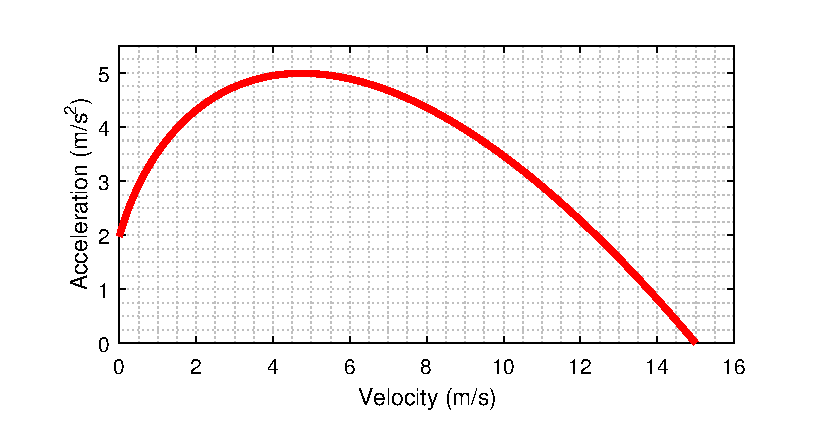
\includegraphics[width=0.9\linewidth]{materials/research_methodology/gipps_2.eps}}
\caption{Relation between available acceleration and current speed for the model derived from Gipps' model. As it can be seen the acceleration drops to zero when maximum speed is reached.}
\label{fig:gipps}
\end{figure} 

As the experiment was dedicated to city traffic the maximum velocity of traditional vehicle was limited to 15 m/s. Starting from full stop and heaving acceleration button pressed the car would reach that velocity after 7.1 seconds.





%show speed/time with full acceleration - compared to autonomous car (or maybe put comparison in autonomous car section)

%graph of coasting...in time or distance travelled - speed vs time?


%gave relatively . 



%However, unlike real car the model used in the simulation 


%Parameters were optimized to give possibly most realistic feeling of car control NFS


%The challenge was to 


%In real car the acceleration is controlled by analogue throttle


%gipps graph here. reference to book or paper?


%gipps

\paragraph{Comparison with autonomous car model}
%this could be seperat subsubsection...?


Figure~\ref{fig:super_graph} compares behaviours of autonomous and traditional car. It can be seen that although profiles have fairly similar shape, there are some significant differences. And so, while traditional car's max speed is higher, its acceleration is slower compared self-driving one. Additionally, braking profile of autonomous car is smoother than human-driven one.

%FIX THIS GRAPH:

\begin{figure}[!] % Example image
\center{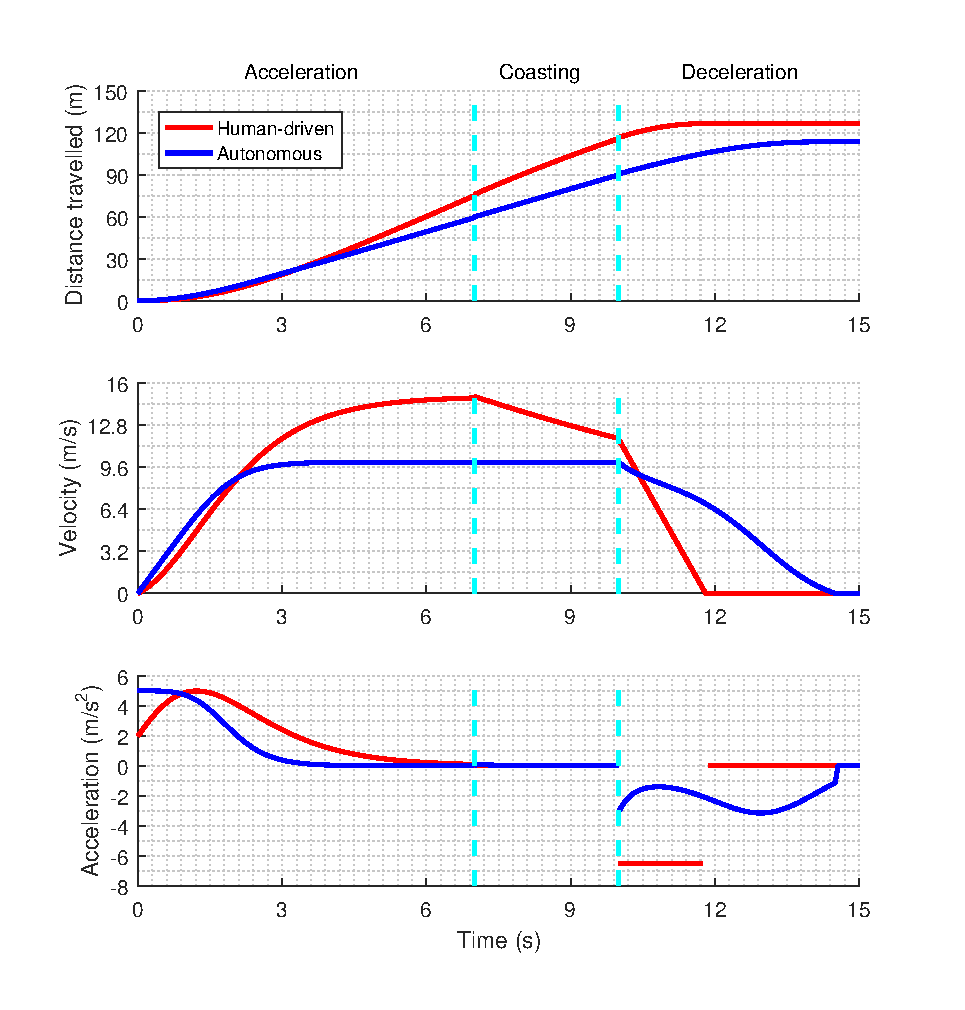
\includegraphics[width=1\linewidth]{materials/research_methodology/super_graph.eps}}
\caption{Behaviour comparison of Autonomous and Human-Driven cars in terms of distance travelled, velocity and acceleration. First section on the left corresponds to both types of vehicles accelerating from zero velocity. Middle section shows coasting when Participant's acceleration is 0 and autonomous car maintains maximum velocity. Section on the right shows Participant slowing down at $-6.5\:\nicefrac{m}{s^2}$ and Autonomous Car detecting stationary object 30 meters ahead.}
\label{fig:super_graph}
\end{figure} 

%super_graph.eps





\subsection{Communication between machines}

One of the key factors contributing to the successful conductance of the experiment was a reliable communication between machines. As it later turned out, it was probably the biggest single challenge of the entire project.
\par
Possible network solutions were considered already at the begging of the project and had significant impact on the choice of primary development environment. Although the exchange of data was one of undependable parts of the project, the way in which communication was established was irrelevant from the point of view of the rest of the software. The network solution was only supposed to meet certain requirements derived from the experiment design.
\par
 After reviewing possible ways of implementation, it was decided to use Robot Operating System which was included in MATLAB's Robotics System Toolbox. Although main intention of ROS was to function as a framework for developing robotics software, it also featured  structured communication solution \citep{quigley2009ros}. From the point of view of the project, ROS could provide reliable, simple to use way of exchanging data. The initial idea was to create one topic for car's location and orientation and another one for orders from participants (Figure~\ref{fig:ros_initial_idea}). 
\par
To justify this approach, a small game was created that exercised almost exactly the same design principle. Performance of the game proved to be satisfactory and the project carried on using this solution. 
\par
However, as the implementation was progressing and tests with multiple clients started, it turned out that subscribing and publishing to the topics takes excessive amount of time and it will be impossible to serve multiple machines and maintain sensible frame rate (which was 20 FPS at that time). In the search for alternative solution other type of ROS communication mechanism was tried which was Services. Nonetheless, this approach proved to be ineffective too. 
\par
After further search a new idea of using User Datagram Protocol emerged. MATLAB provided simple way to establish communication using UDP which proved to be distinctly faster from original idea. Sending 100 bytes of data as a single string lasted around $0.2\:ms$ while receiving took about $3\:ms$. 
In the final network solution UDP was used in conjunction with ROS. UDP provided fast way to send and receive data while ROS allowed to: execute code at fixed rate, synchronize multiple machines to Server's clock and manage overruns if the code execution took too long. 
\par
In order to mitigate the amount of receiving done by the server, an additional entity called Communication Agent was created. This piece of software running on separate machine was responsible for aggregating inputs from all clients, combining them together into one string and sending to Server. The main reason behind this solution was that receiving one long message took less time than receiving multiple short ones. 
\par
Figure~\ref{fig:ros_final} shows what final communication solution looked like. In tests and during the experiment it proved to be reliable and easy to use, albeit with some limitations.

\begin{figure}[!] 
\center{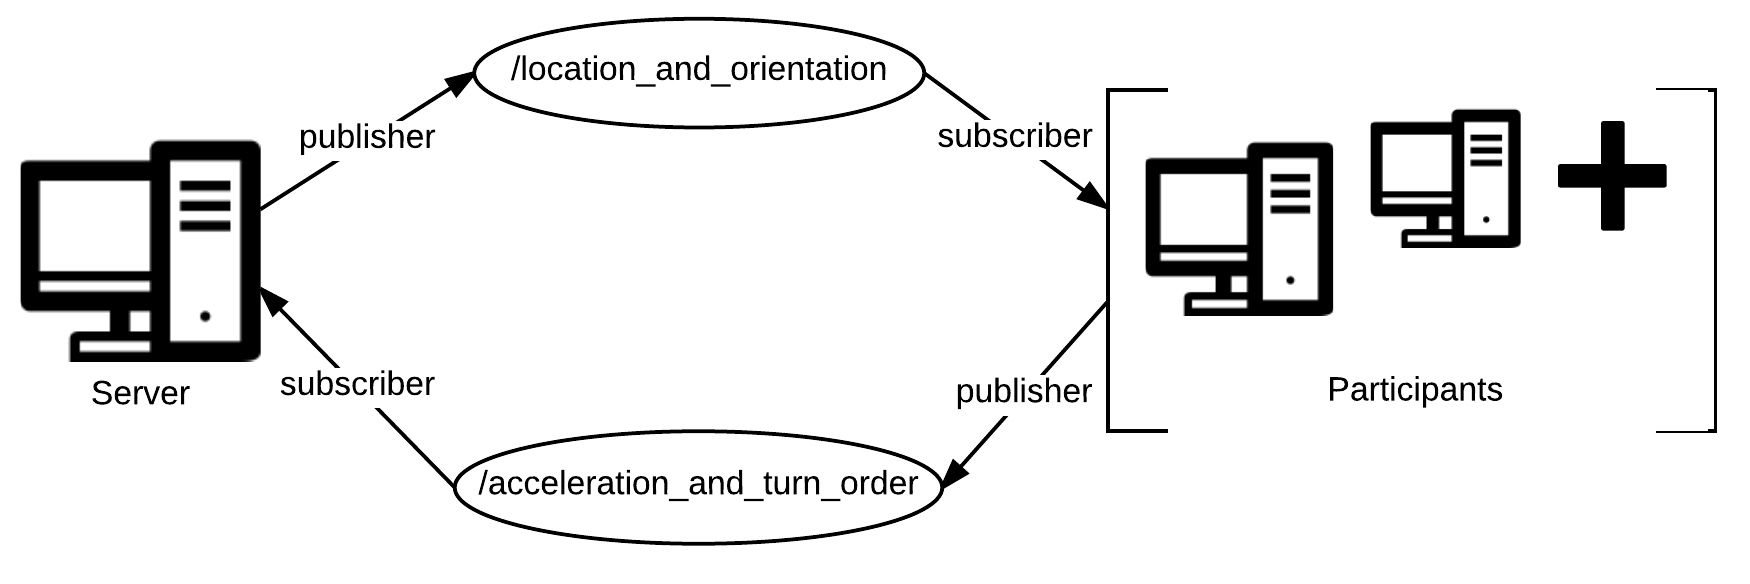
\includegraphics[width=1\linewidth]{materials/research_methodology/ros_initial_idea.png}}
\caption{Initial idea for establishing communication using ROS nodes and topics. It was considered to have only one pair of topics for all participants or individual pair for each single participant.}
\label{fig:ros_initial_idea}
\end{figure} 


\begin{figure}[!] 
\center{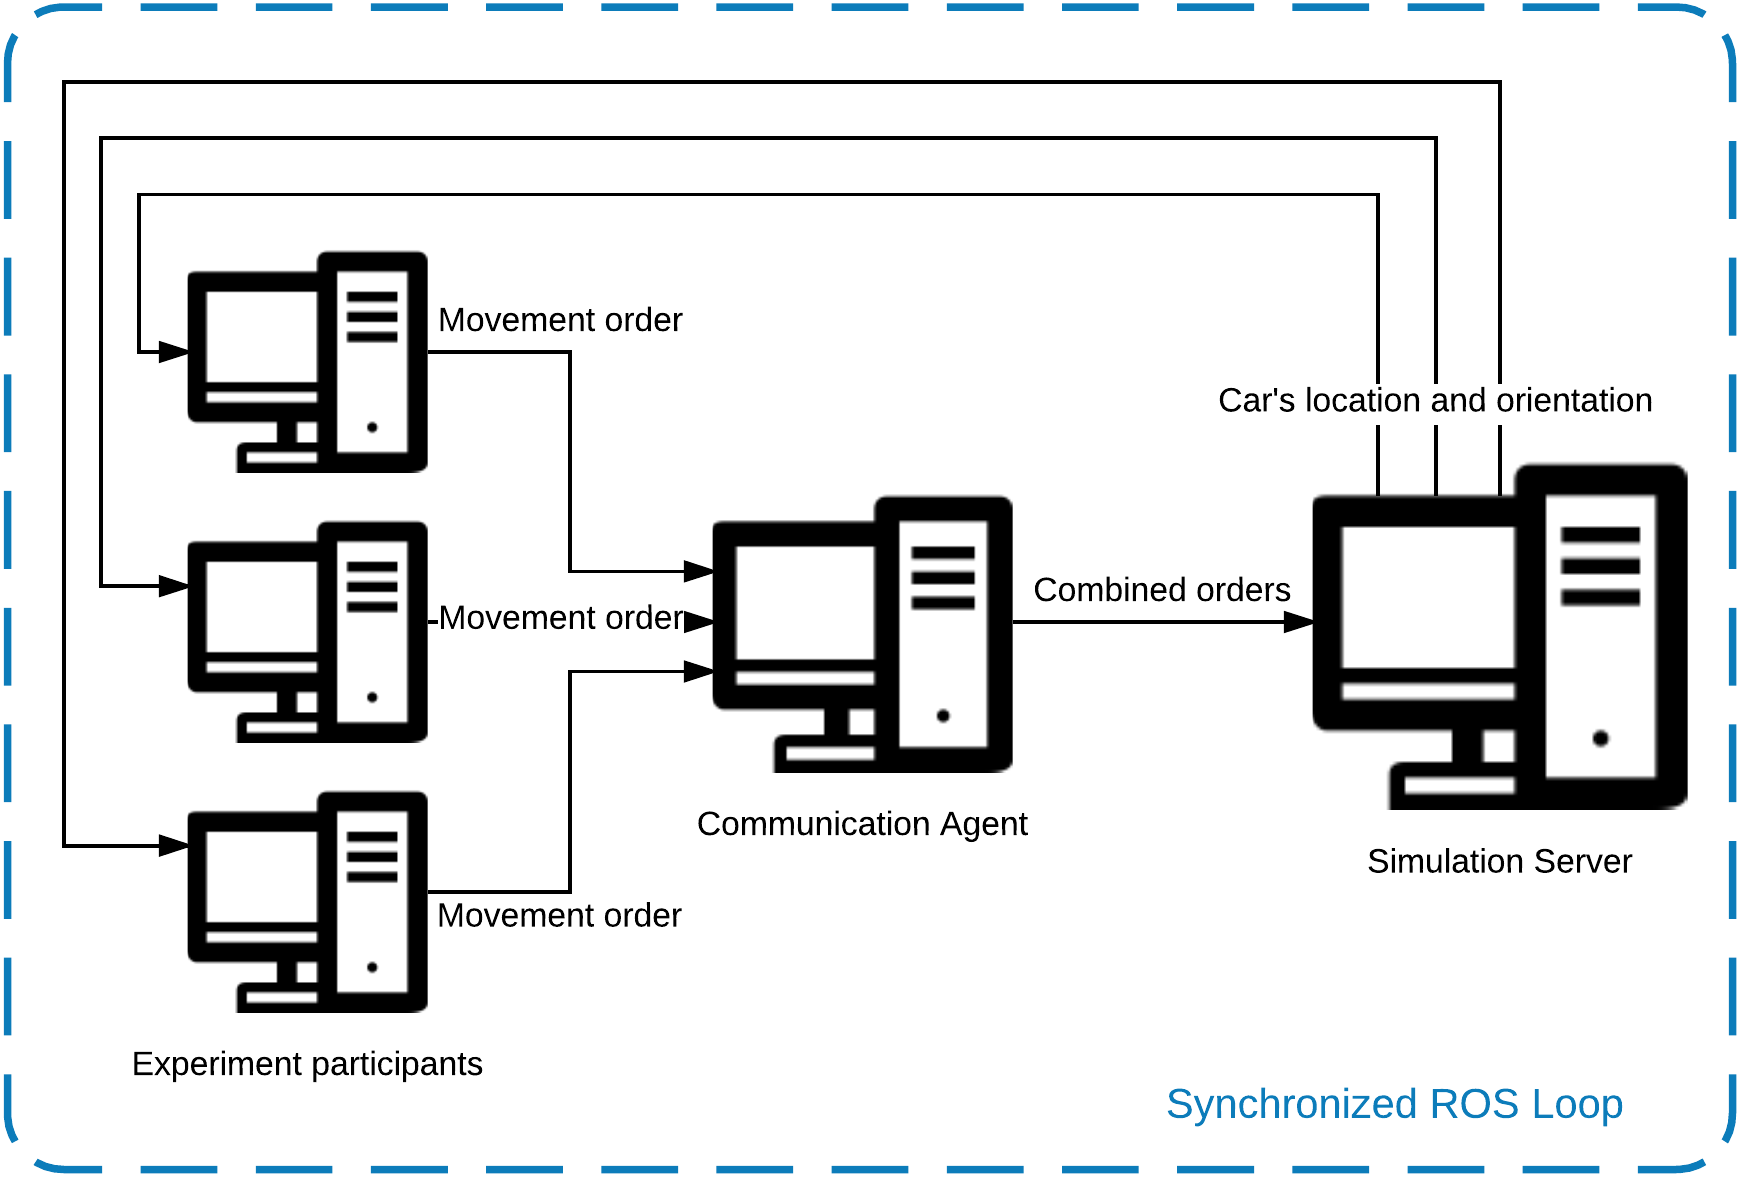
\includegraphics[width=1\linewidth]{materials/research_methodology/ros_final.png}}
\caption{Final communication solution used in the project. A combination of UDP and ROS allowed to have reliable, synchronous exchange of data}
\label{fig:ros_final}
\end{figure} 


\par

The way in which data exchange was implemented was a type of Inter-process communication. According to \citet{rajkumar1995real} this is a considerably challenging task which is often underestimated. Among all objectives that should be met by this kind of  software, the most essential ones are probably reliability and scalability. In the case of this implementation it can be said that communication was very reliable, however not fully scalable as the frame rate was decreasing if there were more than 7 clients connected at the same time \citep{rajkumar1995real}.


\newpage
\section{Experimental Design}

%\paragraph{Experiment design..}

%***add sth about qualitive/quantive method!
The experiment was located at the heart of the project. All work done before was planned for successful delivery of the experiment and all work done afterwards was relying on the data collected during the experiment. 

\par

This chapter is dedicated to the detailed description of the entire experiment. It starts by restating and expanding the principles of the experiment. Then is follows to describe exact configuration of each scenario. Next section describes client's interface and explains reasons standing behind its design. Last part includes responses from questionnaire given to participant and describes exact course of event on the experiment day. 

\par


%\par

\subsection{Principles of the experiment}

This section redefines and expands the guidelines given in Introduction and Motivation chapter.  



%\textbf{style note:} \textit{This is all written in conditional because it was a plan and actual implementation is a different story??}

Final plan for the experiment was to involve around 10 people. Everyone would be asked to control one of the vehicles in the simulation. Each of them would sit in front of a computer where they could use the keyboard and observe the screen. On the screen they would see a top-down view of their own vehicle and it's surrounding. By using the keyboard they would control the acceleration of their vehicle. The instructions given would encourage to explore the map and avoid collisions with other vehicles.

The experiment was planned to consist of three main sessions and one learning session. Each session would feature different scenario which determines road layout, number of human-driven cars and number of autonomous cars. During the preliminary session participants would learn how to control the car, how car responds to their commands,how to turn and what the environment looked like. 
After learning period the first and second phase would commence. Both phases would use identical map but the proportion of traditional cars to autonomous would change. The map shape would be an infinity loop shape where vehicles would have to follow each other and there would be one intersection. It was assumed that such an approach would allow to measure macro parameters of the traffic as both phases would be comparable and the impact of autonomous vehicles could be potentially extracted. The initial choice of measured parameters included average velocity, density, distance covered and other basic statistical parameters such as variance and standard deviation. The scenario in the third phase would use significantly more complex map with 3-way  intersections, road exits and road (accesses?). It would feature a similar number of traditional and autonomous cars. The focus of the analysis would be microscopic interaction between cars in various road situations. 
Number of autonomous vehicles present on the map depended on the number of people turning up for the experiment. Additionally map used for phase one and two could be scaled according to the total number of cars. The instructions given to experiment participants before each phase stated the following:

\begin{enumerate}
  \item Cover as long distance as possible
  \item Avoid collisions with other cars at all cost
  \item Use keys described below to control the car
  \item When given a choice to turn at the intersection it's your decision which direction you want to go
  \item Listen to other instructions
\end{enumerate}

At every step of the simulation all relevant data was recorded for further analysis. In the event of collision the cars would be allowed to pass through each other. None the less, the event was captured and collision alert was displayed for drivers involved in the accident. Collisions were unwanted events that were considered a distortion affecting the results. By allowing the cars to pass, the traffic disturbance was mitigated. Another considered ideas such as teleporting vehicles to another place or manually changing the velocities would probably have greater impact on traffic smoothness. Figure~\ref{fig:gui_4} show a screen-shot of Participant's interface.


\begin{figure}[] % Example image
\center{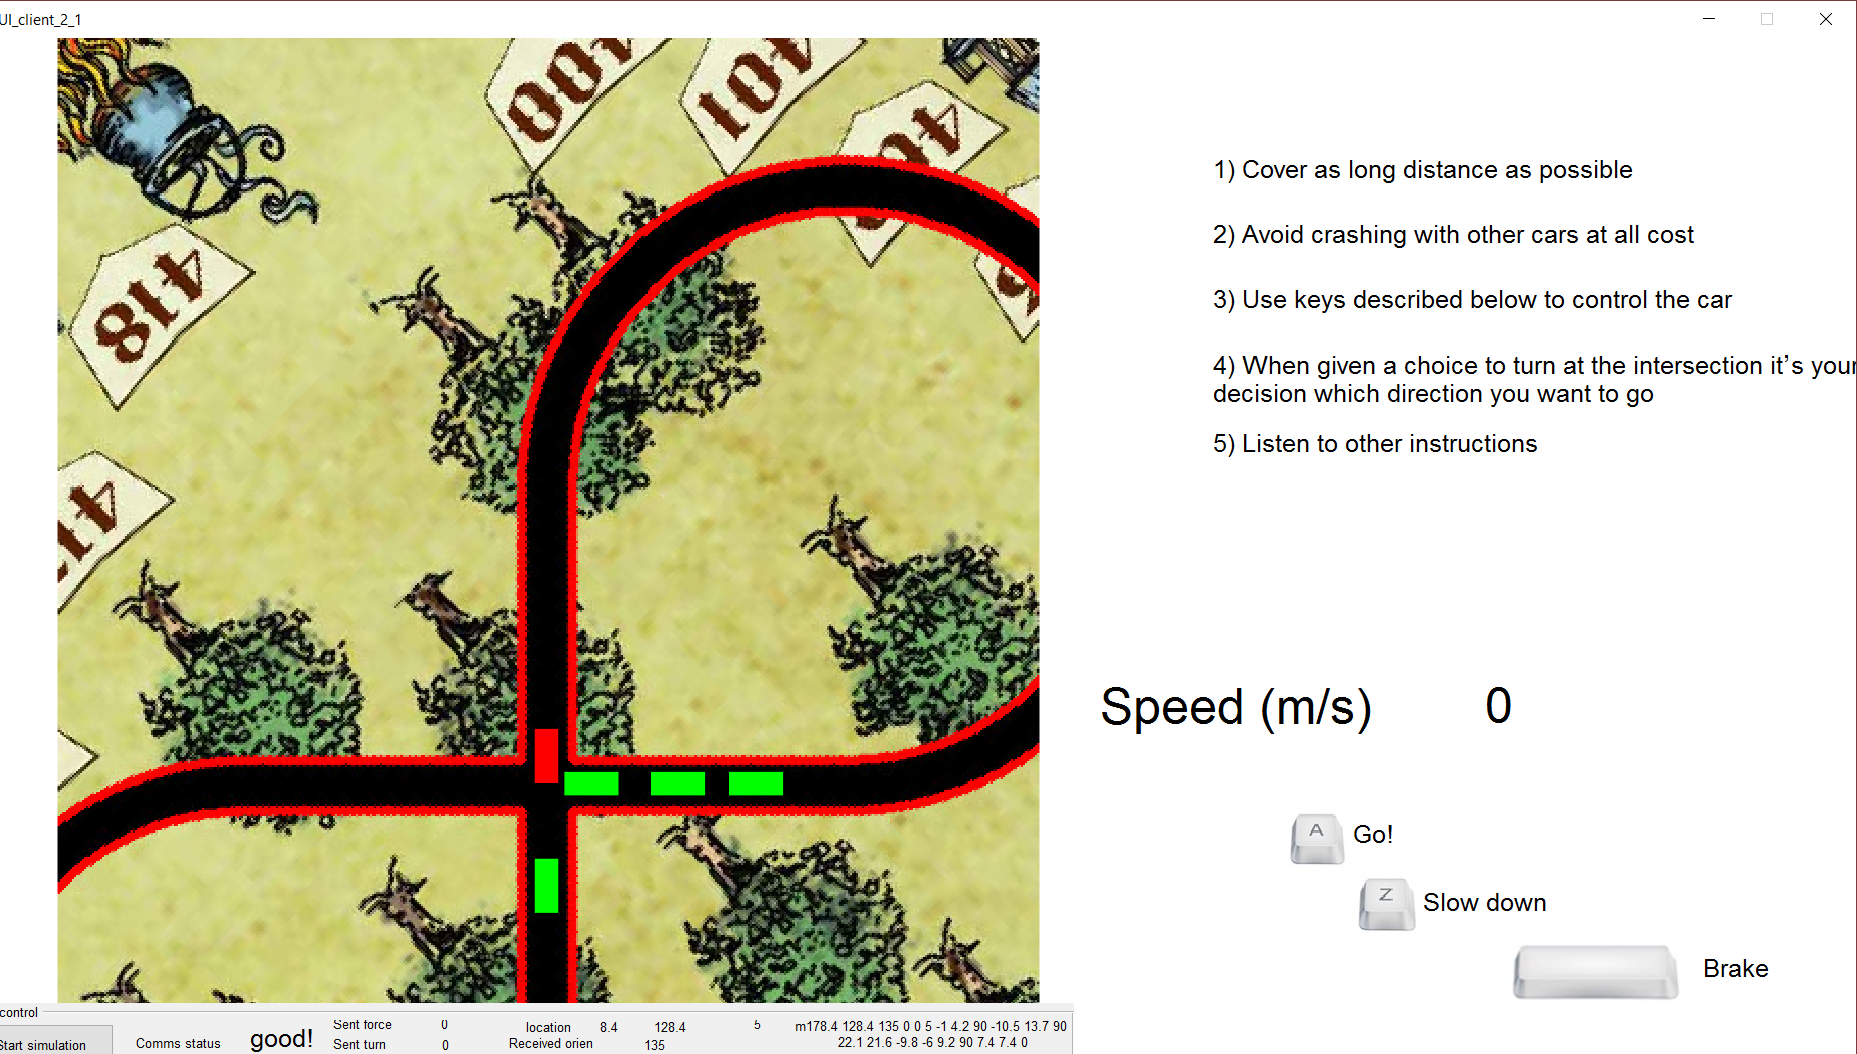
\includegraphics[width=1\linewidth]{materials/research_methodology/gui_4.png}}
\caption{Screenshot of participant's interface. Participant's car is marked in red and all other cars in green. *comment* part of gui is cutted. will fix}
\label{fig:gui_4}
\end{figure}

%The algorithm governing the behaviour of autonomous cars was based on Intelligent Driver Model.  



%(a screenshot from the client gui . Say about control key described, speedometer and collision alert.)









%\paragraph{traffic parameters}

%In order to evaluate traffic performance four key parameters will be measured as suggested in a paper by Beymer and McLauchlan \citep{beymer1997real}. 

%\begin{itemize}
%  \item Flow - Amount of vehicles in one hour (will be separately evaluated for different parts of the track)
%  \item Velocity - Average velocity of individual car or multiple cars
%  \item Density - Amount of vehicles in for specified distance
%  \item Headway - Spacing between vehicles
%\end{itemize}

%Additionally to the parameters above the traffic will be analysed in terms of amount of accidents.



\subsection{Scenarios}

Each scenario specifies configuration of the map, number of human drivers, number of autonomous cars, initial position of each car and length of the simulation. 

While map configuration had to be prepared before, number of vehicles of each type and time of the simulation could be set at the start of the experiment. This flexibility helped to accommodate for unknown number of people that showed up for the experiment. To ensure reasonable congestion but yet high number of interactions each map was designed for different number of vehicles. A benchmark test with solely autonomous cars and additional empirical tests allowed to establish that every vehicle should correspond to 45 to 80 meters of total track length. In all scenarios participants were not told which car is autonomous and which is controlled by another human. They could, however try to guess the type of the car from how it behaved. 

\par
%This section describes initial learning phase and three main phases of the experiment.


\subsubsection{Learning phase}
%\paragraph{Learning how to drive}


The learning period involved all participants and one autonomous car. It lasted 2 to 3 minutes and was intended for getting familiar with the simulation. The data from this period was recorded but was not intended for analysis. In that period participants could ask additional questions. The map used in this scenario is presented on Figure ~\ref{fig:map_0_arrows}.


\begin{figure}[] % Example image
\center{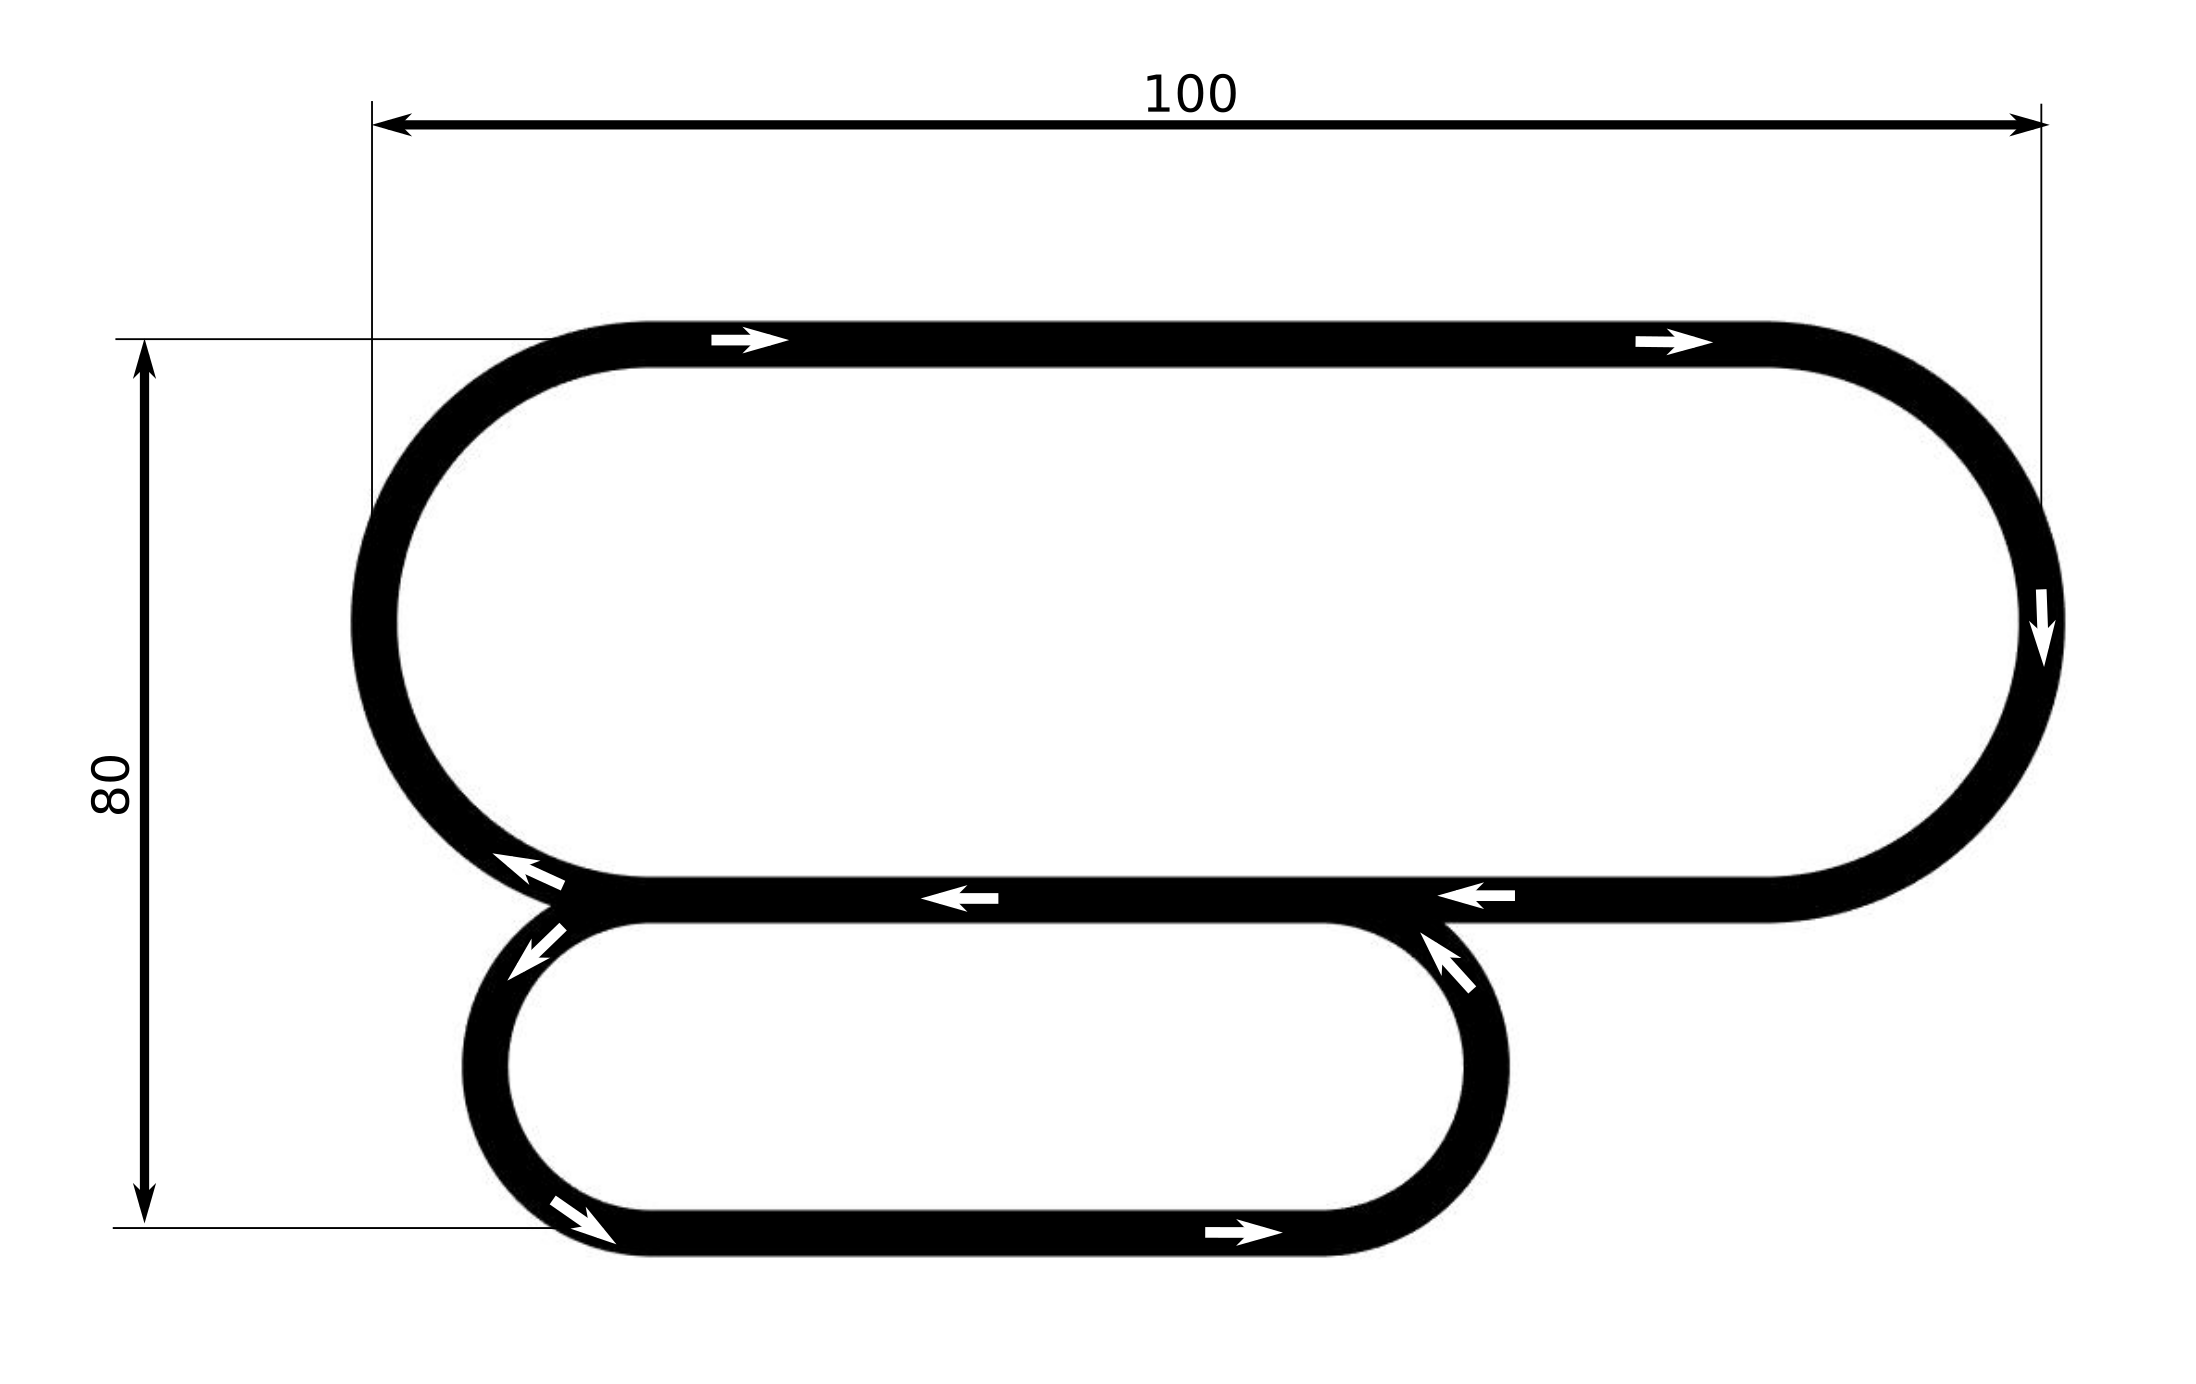
\includegraphics[width=0.8\linewidth]{materials/research_methodology/map_0_arrows.png}}
\caption{Map used in learning scenario. It featured one road exit and one road split. Dimensions are given in meters.}
\label{fig:map_0_arrows}
\end{figure}


\subsubsection{Scenario 1}

In the first scenario all participants were involved and there was one autonomous car. The map featured figure of eight shape as showed on Figure~\ref{fig:map_1_arrows}. The intersection in the middle was uncontrolled as it did not have any priority rule. It was hoped that this way cars would face uncertain situations and interactions will be more vibrant. This scenario was intended to capture interactions in traffic consisting almost entirely of traditional cars. Interactions were either between cars following each other or between cars at the intersection. It was hoped to observe how people are keeping distance to car ahead, how conflicts at intersection are resolved and what are the potential queueing behaviours. Before the simulation started, participants were briefed what is the shape of the map but they were not told how many autonomous cars were in the simulation. This phase was planned to last 4 to 8 minutes depending on the number of participants.
%One autonomous car was added because(why it was added??)

\begin{figure}[] % Example image
\center{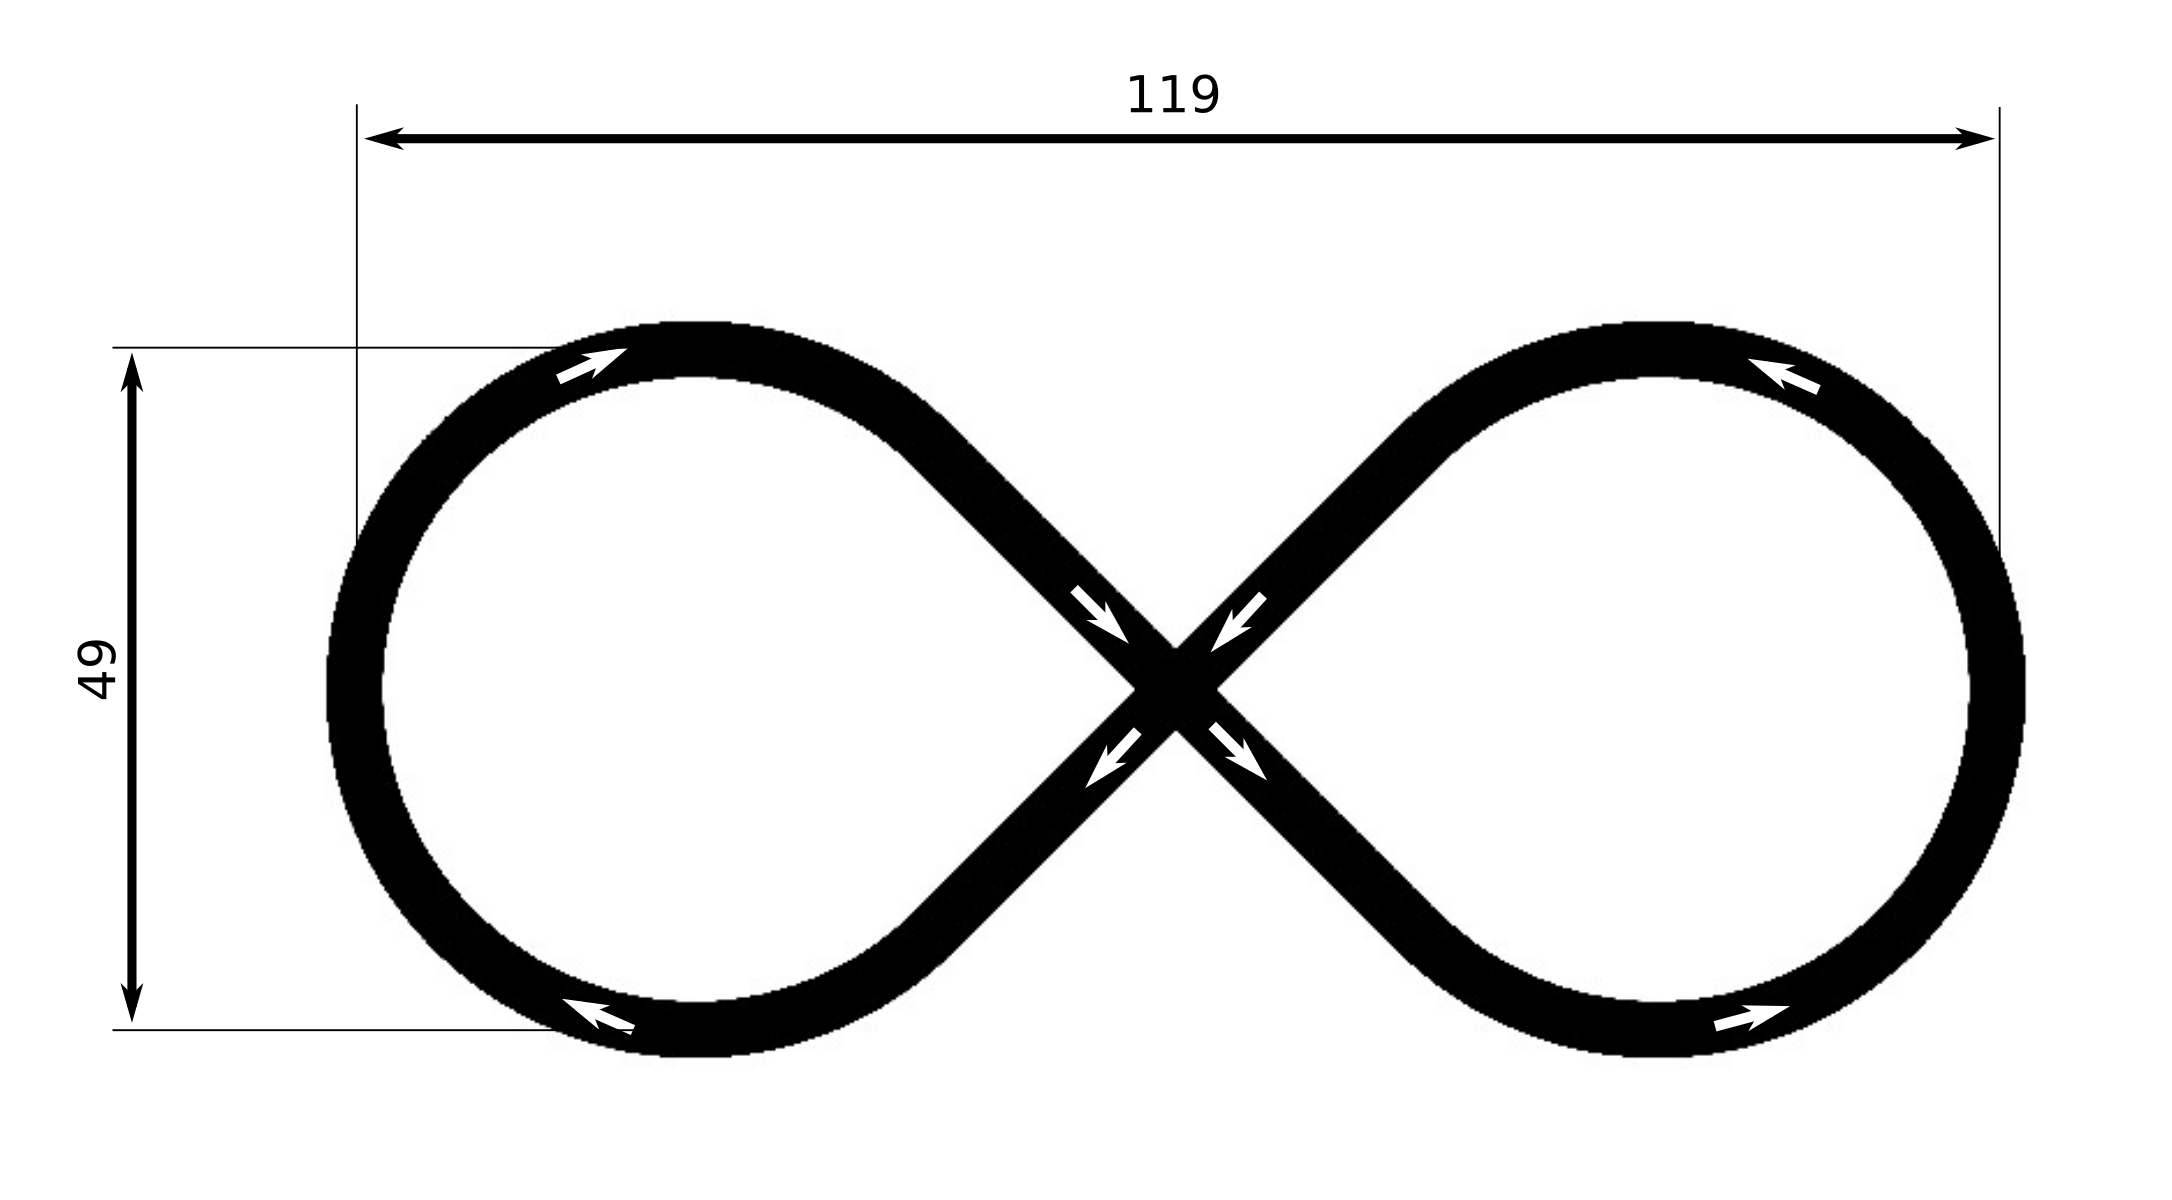
\includegraphics[width=0.8\linewidth]{materials/research_methodology/map_1_arrows.png}}
\caption{Map used in First and Second scenario. It featured infinity loop shape. There were no road splits and cars had to follow each other. Dimensions are given in meters. Covering the whole map at full speed of $15\:\nicefrac{m}{s}$ would take 22 seconds. The track was intended for 6 to 10 vehicles.}
\label{fig:map_1_arrows}
\end{figure}


\subsubsection{Scenario 2}

In scenario 2 around 35\% of people taking part in the first scenario was substituted for autonomous cars. This scenario used identical map as scenario 1 (Figure~\ref{fig:map_1_arrows}) and the total number of cars didn't change. It was hoped that this way the results will be comparable to first scenario. Particular interest was in the interactions at the intersection. The autonomous cars were always letting human-driven cars go first if collision was anticipated. The humans however, didn't know which car is what type and communication happened only via observation of each other's movement. Similarly to previous scenario the planned length would range between 4 and 8 minutes.


\subsubsection{Scenario 3}

Scenario 3 aimed at microscopic interaction between particular pair of vehicles or groups of vehicles. The map used in this scenario featured multiple types of intersections and was much more complex than previous one as it is shown on figure~\ref{fig:map_3_arrows}. The amount of human-controlled cars was equal to the number of autonomous cars. The total density of all vehicles was two times lower than in previous scenarios but due of multiple intersections the number of interactions stayed high.


\begin{figure}[H] % Example image
\center{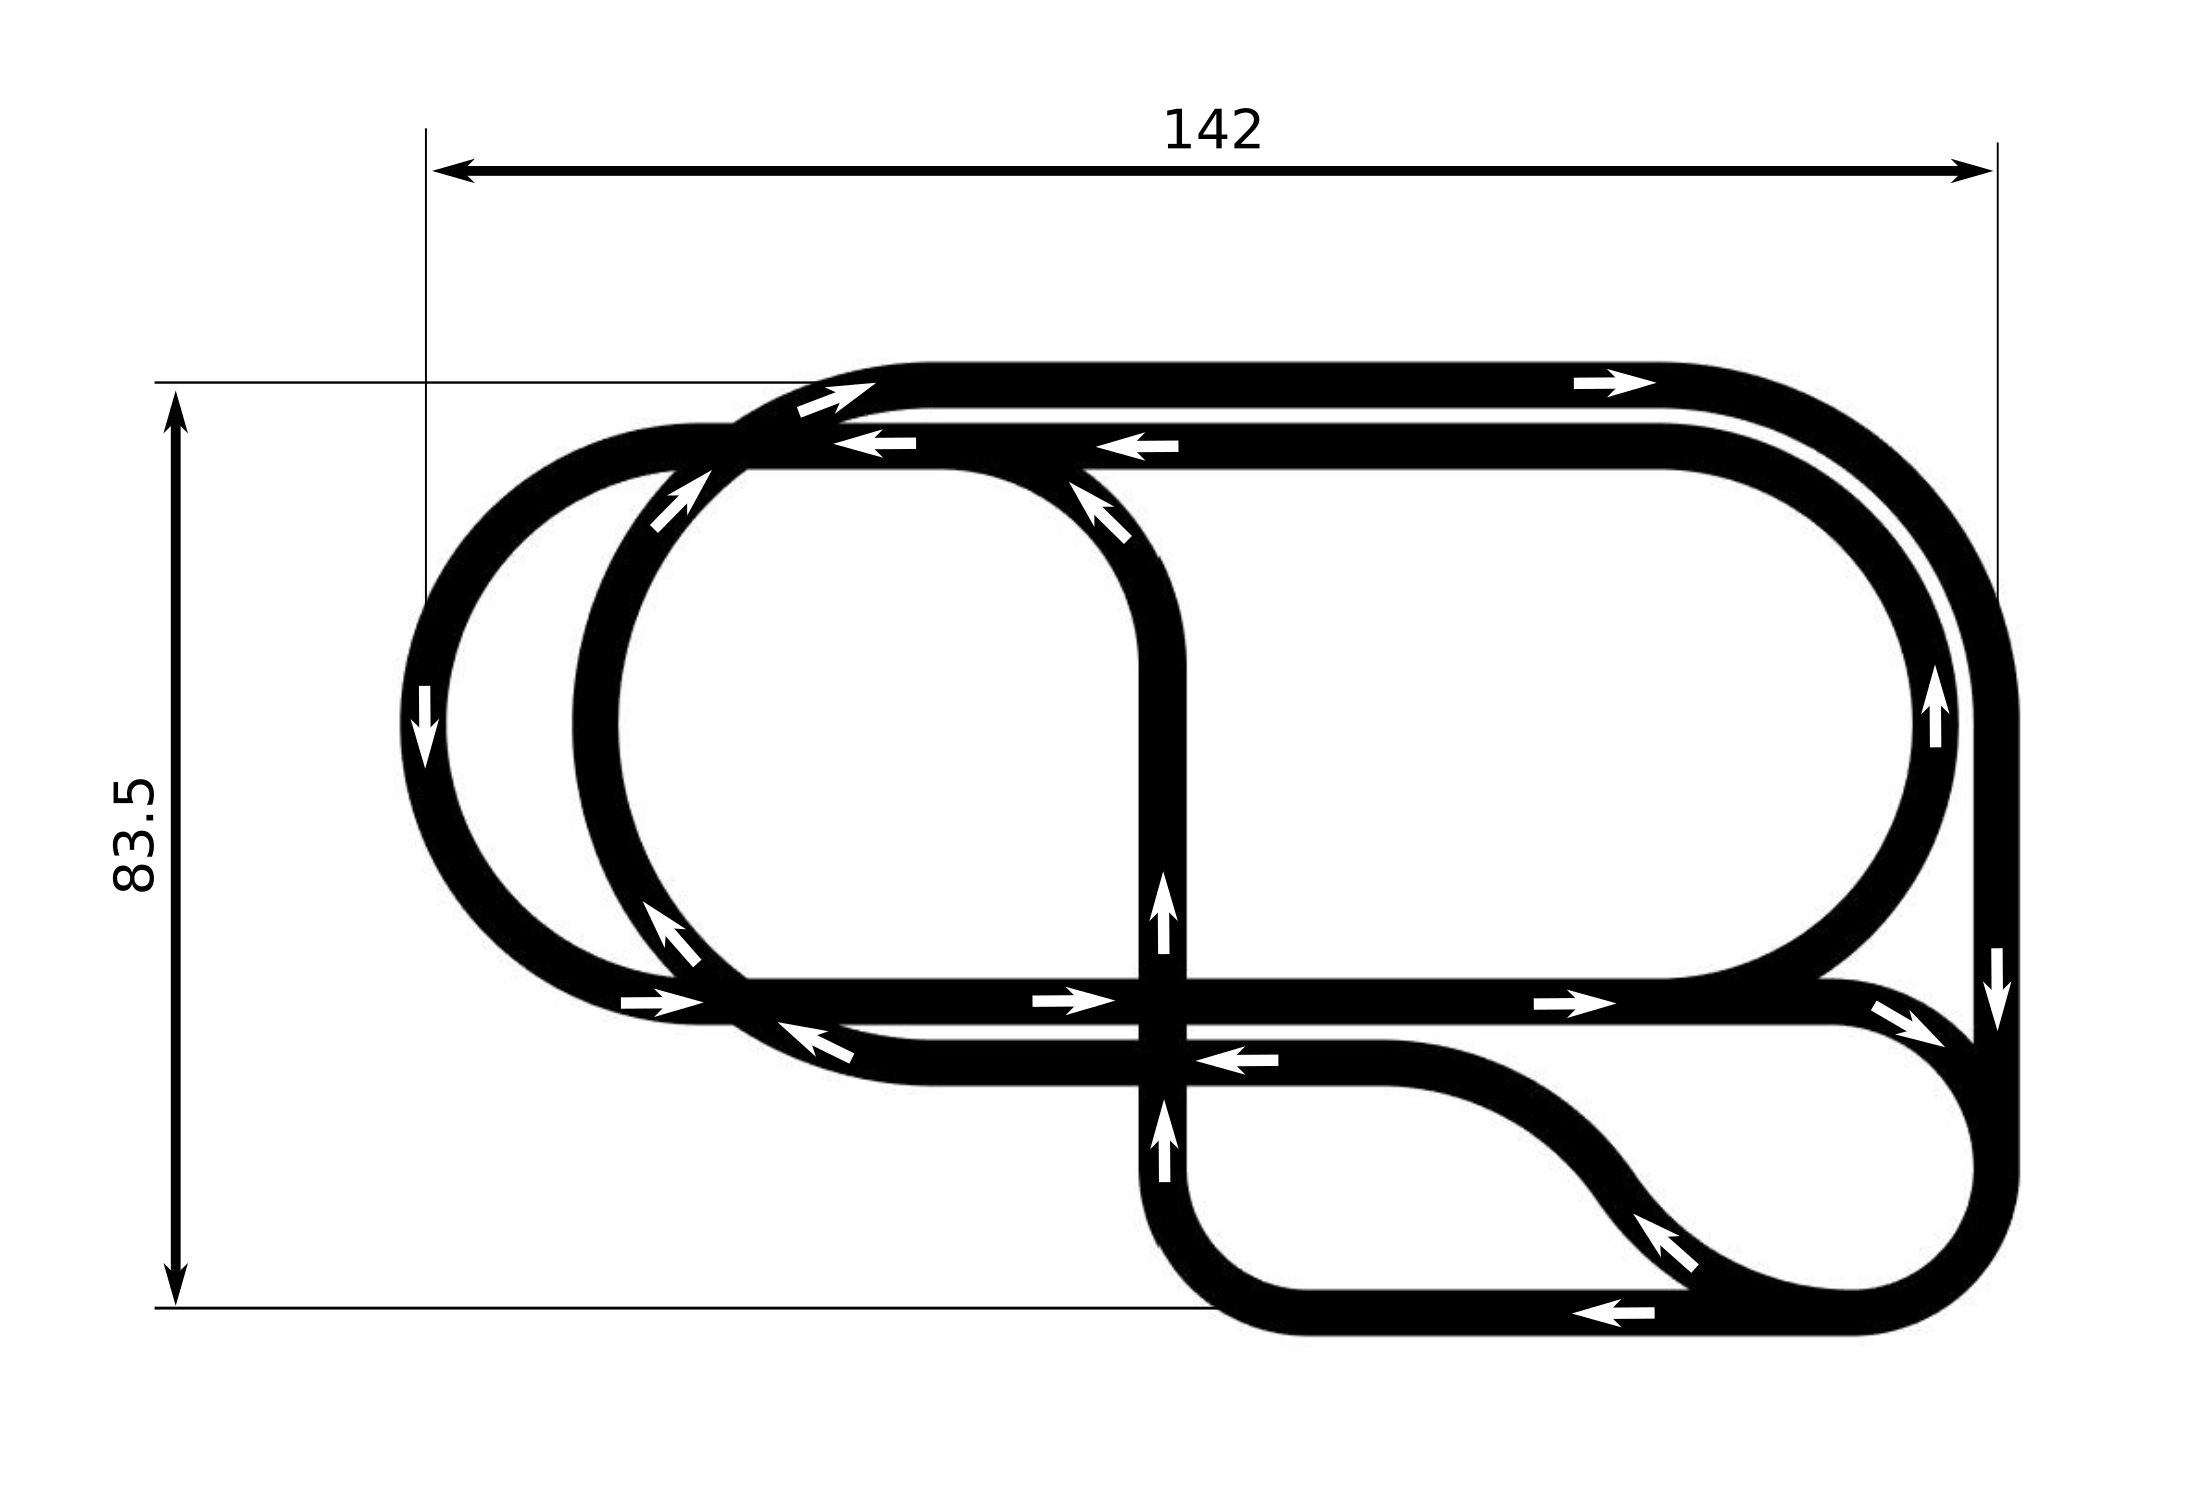
\includegraphics[width=0.8\linewidth]{materials/research_methodology/map_3_arrows.png}}
\caption{Map used in the third scenario. It featured 2 road splits where drivers could change direction, 2 diagonal intersections,a 3-way intersection and 2 road accesses(?). The total length of all segments was 875 m. Travelling at $15\:\nicefrac{m}{s}$ it would take 59 seconds to cover that distance. This was the longest track in the experiment and was designed for 8 to 14 vehicles.}
\label{fig:map_3_arrows}
\end{figure}



\subsection{Client interface}

The main aim of the graphical interface was to mimic what a person driving a car would actually see from the inside of his or her vehicle. Compared to the real world the representation of the environment had to largely simplified. The challenge was to preserve as much of the realism as possible keeping in mind the main principles of the experiment. The cars were represented as coloured rectangles 2 meters wide and 4.5 meters long. Particular participant's vehicle was always position in the middle of the screen while map and other vehicles were moving around it. Roads were 4 meters wide, coloured in black with red boundaries. Each track was overlaid on graphical background with many distinctive features to allow for better sensation of speed (Figure~\ref{fig:gui_4}). Pictire used in the background comes from \citet{sheerwood}.


\paragraph{Car control using keyboard}
First things to decide on was how the car was controlled. Fundamentally the car had one degree of freedom as it always went along a predefined path. Only in the event of road split the driver could make discreet choice on which direction to go. The acceleration of the car was controlled by A and Z keys. Pressing A made car accelerate with a value calculated from Gipps' car following model (discussed later). The maximum velocity was capped at $15\:\nicefrac{m}{s}$. Pressing Z key applied constant deceleration of $-6.5\:\nicefrac{m}{s^2}$. Additionally drivers could press space bar which functioned as a hand break and applied deceleration of $-10\:\nicefrac{m}{s^2}$. These number were found empirically so that car responded predictably. Backward movement was disabled for greater simplification.
The reason for not using arrow keys was that these keys were used to control car's direction as some intersections featured choice between straight, left and right turn. 


\paragraph{Size of view field}
Another design decision concerned the size of driver's view field. The shape and size of the view field was a square 80 meters by 80 meters where car was positioned 20 meters from the bottom as it is showed on previous Figure~\ref{fig:gui_4}. It was assumed that for a driver travelling at full speed it should be possible to comfortably slow down to zero when a stationary vehicle suddenly appears in front of it. The amount of time elapsing from first sight of the obstacle to coming to full stop includes reaction time and breaking time. According to \citep{summala1998driving} average reaction time for a vehicle without brake lights is about 2 seconds which corresponds to 30 meters travelled. Breaking at $-6.5\:\nicefrac{m}{s^2}$ from $15\:\nicefrac{m}{s}$ takes 2.3 seconds which consequently corresponds to 17.2 meters. Therefore minimal distance that driver should be able to see ahead is 47.2 meters. After initial tests this lower-bound value proved to be too small and after few other trials was extended to 60 meters. Another 20 meters of sight distance was added behind the car. 








\subsection{Experiment's execution}

The experiment took place on the 24th of August 2016. 12 people people turned up for the it. The group was divided into 2 smaller groups of 6 people each. Once first group completed all tasks, another one was asked to begin. The reasons to split people into two groups were of technical and research nature. A technical problem arose shortly before the experiment was due to to start. It turned out that from participant point of view the simulation gets considerably laggy if there are more that 7 people playing at the same time. The original frame rate was dropping to few frames-per-second which was unacceptable as it would greatly distort the simulation and whole experiment. From the point of view of experiment methodology heaving two groups conducting identical tasks had beneficial impact on the conclusions that could be drawn from the experiment. It is a common practice to run experiment more than once to detect potential anomalies and have more generalized data(***here use Design and Analysis of Experiments," Handbook of Statistics book).




%%%%%%%%%%%%%%%%%%%%%%%%%%%%%%%%%%%

Experiment was advertised as "Autonomous Cars Simulation". Invitations were sent privately to particular persons. The only information revealed to potential participants stated that experiment will consist of a couple of sessions and they will be asked to drive a car in computer simulation. Participants were promised £10 reward in form of Amazon.com\textsuperscript{\textregistered} voucher and catering available before and after the experiment.


Each of the participants was asked to sit in front of one of selected computers. In front of them there were 3 documents: Consent Form, Participation Information Sheet and Questionnaire. (link to appendixes)
***some more content here
...?

\subsubsection{Questionnaire}

Each of the participants was asked to complete short questionnaire. (link to appendixes). The purpose of the questionnaire was to collect data that later could be used in association with experiment results to create a driving profile for particular person. The exact way in which this data will be used in analysis was not established before the experiment. None the less, it was attempted to ask about things that could be associated with performance of each person.

The survey consisted of 12 questions which can be divided into 4 sections. There were 2 questions asking about gender and age. Next it was asked whether a person played any racing computer games and is familiar with controlling the car with arrow keys. The third section was conditional to the possession of driving licence. If the answer was affirmative, further questions asked about past accidents, subjective evaluation of person's driving style and irritating behaviours they encounter of the roads.
Last question asked about opinion on how the traffic will change when autonomous cars are introduced. 




\subsubsection{Minutes}

The experiment started by reading the Participation Information Sheet to all participants. First paragraph stated rights of experiment participants and how the collected data will be used. Second one explained the task in short and concise way. The exact instructions that were given stated as follows:

"\textit{If you decide to take part in the study, you will be asked to drive a car in on-line traffic simulation. You will be using computer keyboard to control your car. Your main objectives is to cover as long distance as possible and avoid crashing into other cars. There will be 3 phases. Each will last 8 minutes, feature different map and different amount of autonomous vehicles. First phase will be preceded with 3-minute- long learning period when you will be able to learn how to play the game. All additional instructions will be given to you before each phase in form of power point slides. Before starting the simulation you are asked to complete a short survey to describe your driver profile.}"

Rest of the document considered health warnings such as epilepsy and past accidents. Next, participants were asked to complete the Questionnaire described above and sign the Consent form. Once that was done they were told once again what is their task, how to control the vehicles and what the next phase will look like. Eventually the main part of the experiment commenced. It consisted of consecutive phases as described it table \ref{table:minutes_table}.


\begin{table}[h]
\centering
\begin{tabular}{|c|c|c|c|c|}
\hline
\textbf{Phase} & \textbf{Scenario} & \textbf{Human-driven vehicles} & \textbf{Autonomous vehicles} & \textbf{Lenght} \\ \hline
\multicolumn{5}{|c|}{\textbf{Group 1}}                                                                               \\ \hline
Learning       & Learning          & 6                              & 1                            & 1:45 min        \\ \hline
1              & Scenario 1        & 6                              & 1                            & 3:22 min        \\ \hline
2              & Scenario 2        & 4                              & 3                            & 4:12 min        \\ \hline
3              & Scenario 3        & 4                              & 4                            & 4:09 min        \\ \hline
\multicolumn{5}{|c|}{\textbf{Group 2}}                                                                               \\ \hline
Learning       & Learning          & 6                              & 1                            & 4:33 min        \\ \hline
1              & Scenario 1        & 6                              & 1                            & 4:07 min        \\ \hline
2              & Scenario 2        & 4                              & 3                            & 5:03 min        \\ \hline
3              & Scenario 3        & 4                              & 4                            & 4:51 min        \\ \hline
4 (additional) & Scenario 3        & 6                              & 4                            & 2:24 min        \\ \hline
\end{tabular}
\caption{My caption}
\label{table:minutes_table}
\end{table}

The lengths of each phase were considerably shorter than planned. The initial schedule, however, did not account for heaving two streams of people. After the main part of the experiment finished, participants were debriefed and invited for catering. Entire experiment lasted around 1.5 hours and in total 31 minutes of simulation data were harvested.










\section{Results}

\paragraph{}

%...another sentence here
The analysis of the data could be divided into two parts. First one is dedicated to finding patterns, observing dependencies and evaluating particular group and participants. Second one proposes a range of hypotheses which were consequently tested to prove them right or deny. %The discussion of the results was placed in next chapter.

%***DRAFT***
\par

Data collected during the experiment was considerably rich in features and lots of regularities could be potentially found. On average, participants changed acceleration/deceleration commands 73 times per minute. 
Figure~\ref{fig:sample_snapshot} shows a snapshot from the simulation playback.  
 
 
\begin{figure}[h] % Example image
\center{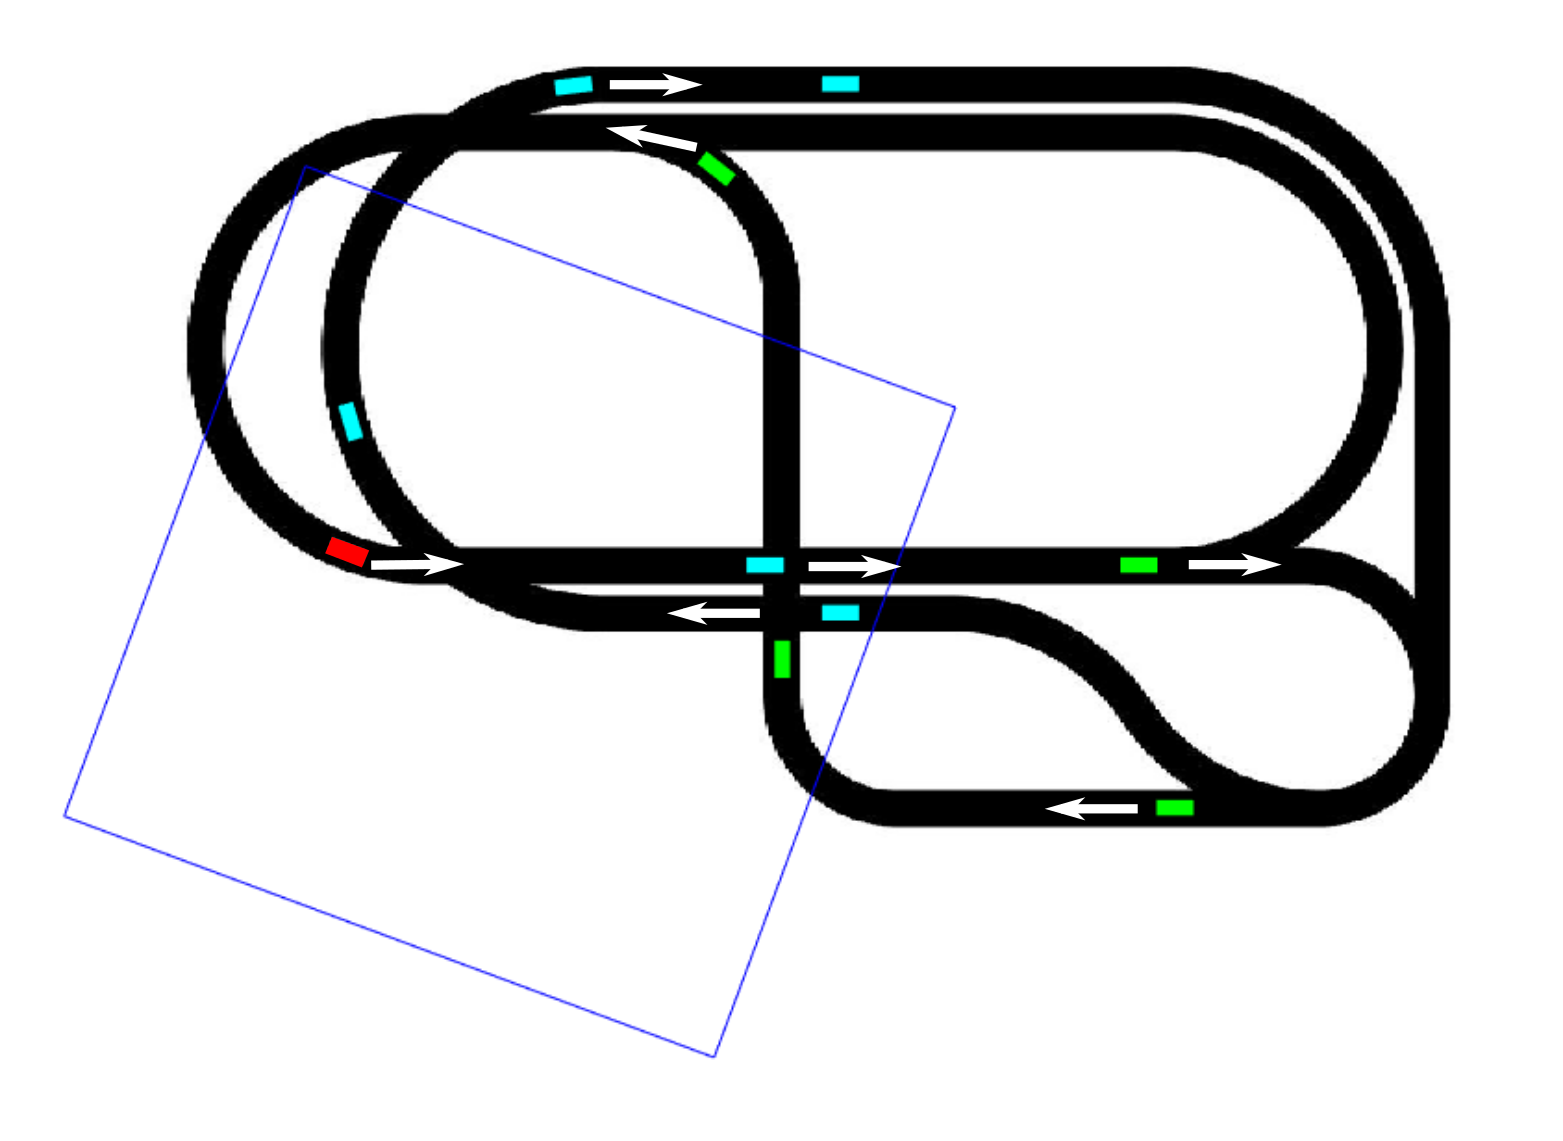
\includegraphics[width=1\linewidth]{materials/findings_and_results/sample_snapshot2_2.png}}
\caption{Group 2, phase 3. A snapshot from simulation playback. Cyan colour represents human-driven cars and green represents autonomous cars. A dark blue rectangle represents the what area was visible for the car marked in red colour.}
\label{fig:sample_snapshot}
\end{figure} 
 
the initial choice of parameters measured across data set was different from what different from what was calculated in the process of the data analysis.



\subsection{Observations}


\paragraph{}

During project's design stage it was very uncertain what kind of results could be expected. Only during the development stage and after the experiment certain ideas on what patterns in data might be observed were established. This chapter proposes three different observation that are aimed at presenting the outline of the collected data. 


%The ideas for different approaches to data analysis formed mainly after the experiment itself



%***some introduction to chapter here



%Say about flaws of autonomous car



\subsubsection{Deceleration mapping}
\paragraph{}

First concept that could help to understand the data, was to visualize how vehicles accelerated and decelerated. In order to do that, a spatial representation of average decelerations was created, as it it shown of Figure~\ref{fig:decelerations1}. Track was divided into 4-meters-long segments and for each segment the total value of decelerations was summed up over all vehicles and all frames in the current phase. Results were plotted for first and second scenario for group 1.


\begin{figure}[h]
\centering
\subfloat[Group 1, Scenario 1]{%
  
\includegraphics[clip,width=0.8\linewidth]{materials/findings_and_results/deceleration_scenario_1_group_1.eps}%
}

\subfloat[Group 1, Scenario 2]{%
  
\includegraphics[clip,width=0.8\linewidth]{materials/findings_and_results/deceleration_scenario_2_group_1.eps}%
}

\caption{Visual representation of decelerations on map used in first and second scenario. Dark blue represents strong deceleration while light yellow represents weak deceleration. The data was averaged over all vehicles including human-driven and autonomous one.}
\label{fig:decelerations1}
\end{figure}

It can be observed from the plot that once multiple autonomous cars were introduced, vehicles decelerated harder and more often when approaching the intersection.




%later: possible reasons: interactions HA were worse



\subsubsection{Evaluation of participant's performance}
\paragraph{}

the number of collisions caused by each participant was evaluated and compared against the questionnaire responses. Single collision always involved 2 cars. A person responsible was always the one whose car's front line intersected with the other car first. A number of collisions caused by each person is shown on Figure~\ref{fig:collisions_total}. Table~\ref{table:collisions_table} shows number of collisions against questionnaire responses. Because the shorter phase lasted 3:22 minutes, values were calculated only for that period for all phases. From these figures it can be seen that:
\begin{itemize}
  \item Almost every person in the first group performed significantly better in terms of number of collisions than participants from the second group. Because of this reason first group was used more often in further analysis as a sole source of data.
  \item Autonomous cars were responsible for only one collision throughout the entire experiment. 
  \item  In total 52 collisions occurred between two human drivers while 33 happened between human drivers and autonomous vehicles. However, accounting for how much each vehicle spent on the track .... ?
\end{itemize}



%***DRAFT***

%HH and HA collisions..?

%In order to decide who was responsible for

%Performance of each participants was evaluated on the basis of 


%Heaving two groups of people allowed to find potential anomalies..

%asses every participants:


\begin{figure}[h] % Example image
\center{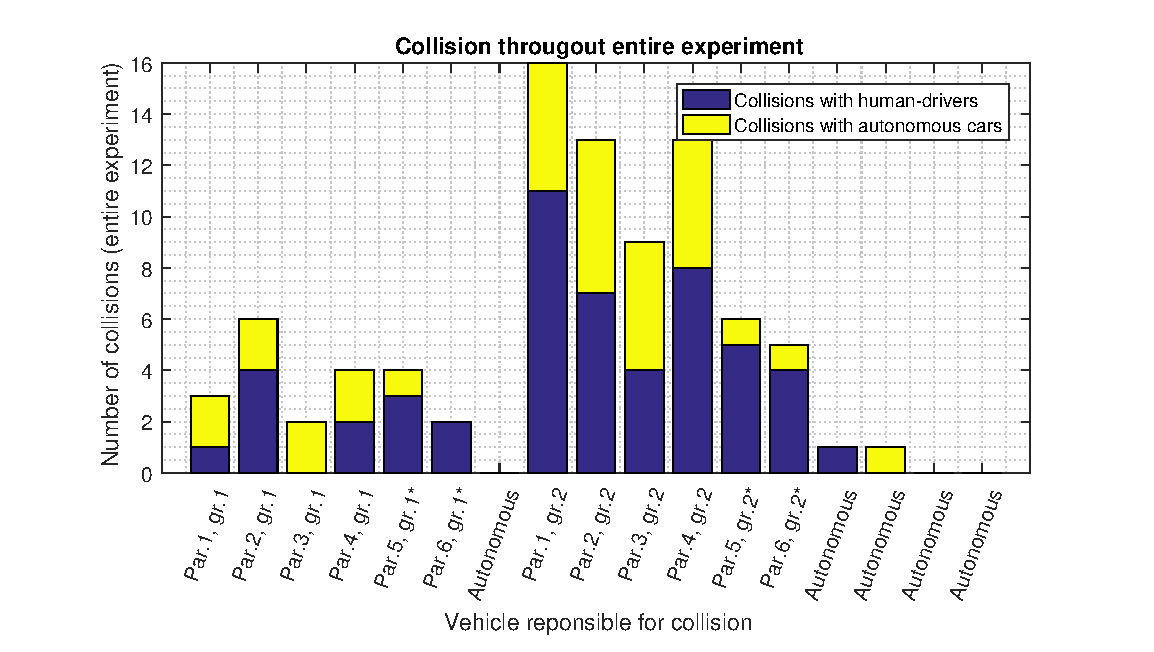
\includegraphics[width=1\linewidth]{materials/findings_and_results/collisions_total.eps}}
\caption{Number of collisions caused by each participant/vehicle in first and second group. (*Humans substituted for autonomous cars in later phases.)}
\label{fig:collisions_total}
\end{figure}





\begin{table}[]
\centering
\begin{tabular}{|c|c|c|c|c|c|c|}
\hline
\textbf{\begin{tabular}[c]{@{}c@{}}Partici-\\ pant\end{tabular}} & \textbf{\begin{tabular}[c]{@{}c@{}}Familiar with \\ keyboard car \\ control?\end{tabular}} & \textbf{\begin{tabular}[c]{@{}c@{}}Years of\\ driving\\ experience\end{tabular}} & \textbf{\begin{tabular}[c]{@{}c@{}}Past \\ accidents\end{tabular}} & \textbf{\begin{tabular}[c]{@{}c@{}}Driving \\ skill \\ evaluation*\end{tabular}} & \textbf{\begin{tabular}[c]{@{}c@{}}Driving \\ style**\end{tabular}} & \cellcolor[HTML]{C0C0C0}{\color[HTML]{000000} \textbf{\begin{tabular}[c]{@{}c@{}}Collisions \\ (H/A)\end{tabular}}} \\ \hline
\multicolumn{7}{|c|}{\textbf{Group 1}}                                                                                                                                                                                                                                                                                                                                                                                                                                                                                                              \\ \hline
1                                                                & Yes                                                                                        & 2                                                                                & 0                                                                  & 2                                                                                & Very careful                                                        & \cellcolor[HTML]{C0C0C0}{\color[HTML]{000000} \textbf{1/2}}          \\ \hline
2                                                                & Yes                                                                                        & 1                                                                                & 1                                                                  & 8                                                                                & Careful                                                             & \cellcolor[HTML]{C0C0C0}{\color[HTML]{000000} \textbf{4/2}}          \\ \hline
3                                                                & Yes                                                                                        & 5                                                                                & 0                                                                  & 8                                                                                & Normal                                                              & \cellcolor[HTML]{C0C0C0}{\color[HTML]{000000} \textbf{0/2}}          \\ \hline
4                                                                & Yes                                                                                        & 6                                                                                & 0                                                                  & 9                                                                                & Careful                                                             & \cellcolor[HTML]{C0C0C0}{\color[HTML]{000000} \textbf{2/2}}          \\ \hline
5                                                                & Yes                                                                                        & 5                                                                                & 2                                                                  & 7                                                                                & Careful                                                             & \cellcolor[HTML]{C0C0C0}{\color[HTML]{000000} \textbf{3/1}}          \\ \hline
6                                                                & Yes                                                                                        & 2                                                                                & 2                                                                  & 10                                                                               & Normal                                                              & \cellcolor[HTML]{C0C0C0}{\color[HTML]{000000} \textbf{2/0}}          \\ \hline
\multicolumn{7}{|c|}{\textbf{Group 2}}                                                                                                                                                                                                                                                                                                                                                                                                                                                                                                              \\ \hline
1                                                                & Yes                                                                                        & No licence                                                                                & -                                                                  & -                                                                                & -                                                                   & \cellcolor[HTML]{C0C0C0}{\color[HTML]{000000} \textbf{11/5}}         \\ \hline
2                                                                & Yes                                                                                        & 3                                                                                & 1                                                                  & 9                                                                                & Normal                                                              & \cellcolor[HTML]{C0C0C0}{\color[HTML]{000000} \textbf{7/6}}         \\ \hline
3                                                                & Yes                                                                                        & 8                                                                                & 0                                                                  & 8                                                                                & Careful                                                             & \cellcolor[HTML]{C0C0C0}{\color[HTML]{000000} \textbf{4/5}}          \\ \hline
4                                                                & Yes                                                                                        & 15                                                                               & 3                                                                  & 10                                                                               & Normal                                                              & \cellcolor[HTML]{C0C0C0}{\color[HTML]{000000} \textbf{8/5}}         \\ \hline
5                                                                & Yes                                                                                        & 8                                                                                & 2                                                                  & 8                                                                                & Agressive                                                           & \cellcolor[HTML]{C0C0C0}{\color[HTML]{000000} \textbf{5/1}}          \\ \hline
6                                                                & Yes                                                                                        & 3                                                                                & 0                                                                  & 1                                                                                & Very careful                                                        & \cellcolor[HTML]{C0C0C0}{\color[HTML]{000000} \textbf{4/1}}          \\ \hline
\end{tabular}
\caption{Questionnaire responses represented against number of collisions caused by each person. It can be observed that self-assessment of driving did not correspond to the number of accidents. (*Own judgement of driving skills on the scale from 1 to 10. **Own judgement of driving style from very careful to very aggressive. Please refer to appendix for details.)}
\label{table:collisions_table}
\end{table}




\subsubsection{Conflicts resolution}
\paragraph{}
Interactions between cars can be systematized as one car following another or as a broad range of interactions at intersections. The later was of particular interest because of it's uncertainty and unpredictability. While all maps featured intersections, figure of eight map used in first two scenarios was aimed at more organized analysis and will be used in this example to visualize how humans and autonomous cars made decisions. Figure~\ref{fig:interactions_example_1v2} shows an example of interaction between one human-driven and two autonomous car. In this example both vehicles at the front came to full stop. In the ideal situation one vehicle should pass while the other slows down.

%***//something on conficts reosultion: some paper/ nash equlibrum
%some paper on interaction between autonomous cars



\begin{figure}[!] % Example image
\center{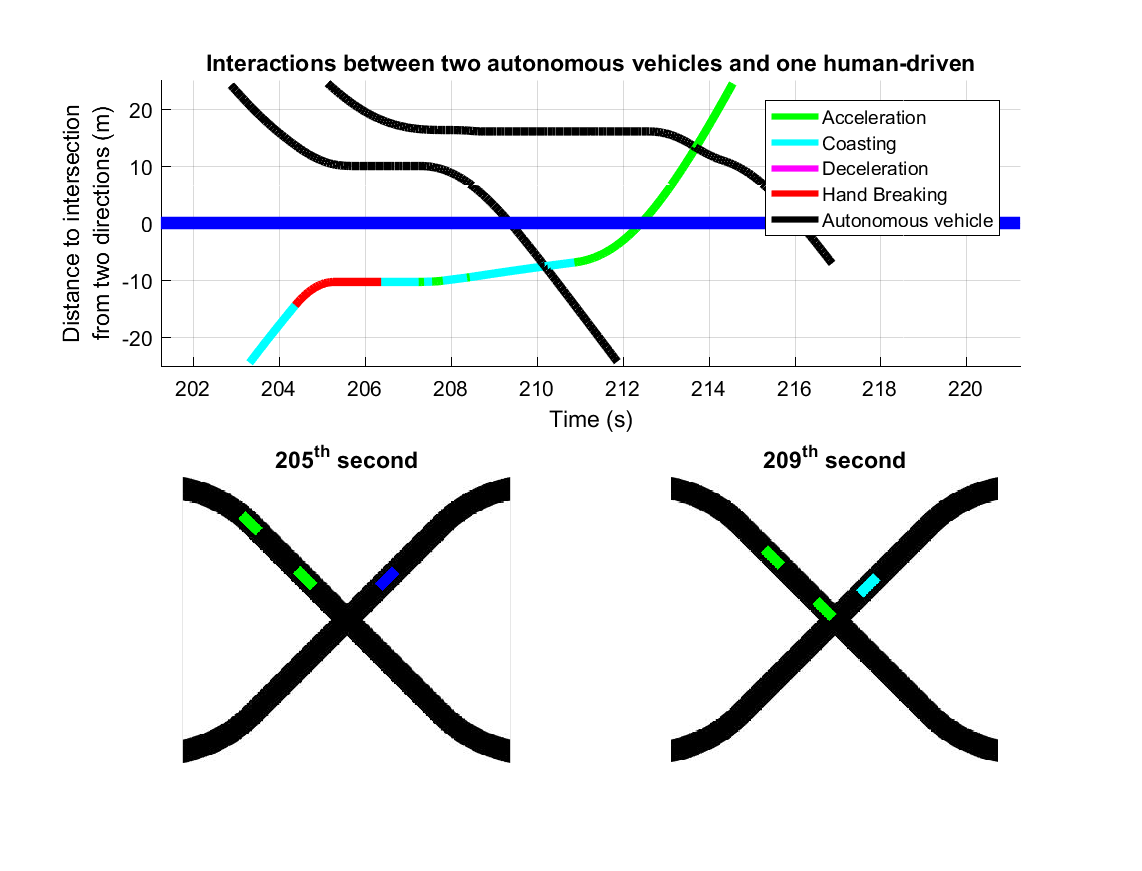
\includegraphics[width=1\linewidth]{materials/findings_and_results/interactions_example_1v2.eps}}
\caption{An example of interaction between two autonomous vehicles and one human-driven. In the 204\textsuperscript{th} second both cars started to brake to avoid collision and came to full stop. Human driver was uncertain of how the other car will behave. Autonomous car, on the other hand calculated collision free passage as other vehicle was not moving and starter to move through the intersection in the 208\textsuperscript{th} second. Next, the human passed through and another autonomous vehicle afterwards. (Colours indicate current order from Participant.)}
\label{fig:interactions_example_1v2}
\end{figure}

Another type are interactions between two autonomous cars as it is shown in Figure~\ref{fig:interactions_example_2}. When two autonomous cars anticipate collision with each other the one which is slower is ordered to reduce its speed according to the time-to-collision value while the faster one passes through uninterrupted. In most cases, this relatively simple rule optimizes the interaction reducing braking to minimum.  




%interactions_example_2

%//figure of autonomous cars

\begin{figure}[!] % Example image
\center{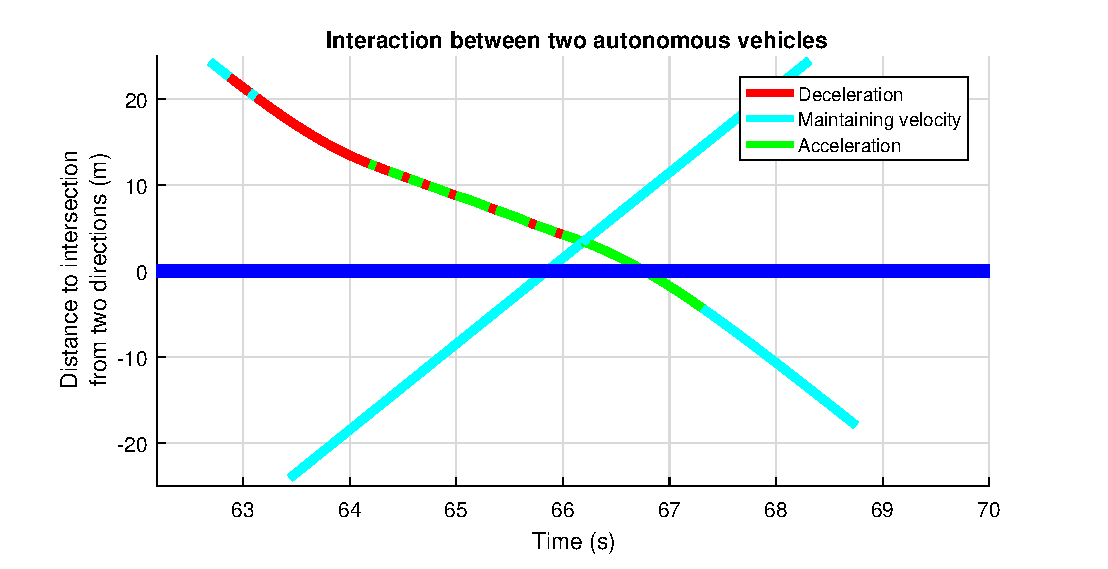
\includegraphics[width=1\linewidth]{materials/findings_and_results/interactions_example_2.eps}}
\caption{An example of interaction at the intersection between two autonomous vehicles coming from different directions. Both cars anticipated collision in the 65\textsuperscript{th} second. In line with the algorithm the slower car started to decelerate as much as it was needed to avoid collision. At each time step new time-to-collision was calculated and velocity adjusted accordingly. The faster car's velocity remained constant.}
\label{fig:interactions_example_2}
\end{figure}





%\subsubsection{Reaction times}


%Another topic of interest were reaction times of both types of vehicles. It was anticipated that the rule to always let human driver pass first and potentially faster reaction by autonomous car would have beneficial impact on the traffic. Particular interest was in differences between reaction times of humans and autonomous cars.

%***//use third map here akso...





%\subsubsection{***other observations..(TO DO)}


%interactions_example_1
%***DRAFT***

%also exmaple of two autonomous cars and two human drivers



%part 1: observations:
%some interesting graph but no broad idea what for :D

%-evaluate group (in terms of number of accidents, questionnaire responses) and which group were in general better - that will justify why you use one group more often

%- 

%- heatmap of accelerations in figure of eight for two phases...and two groups?
%also scenario 3




%scenario 1 and 2 (from different groups):
%- your nice graph with lines for some h-h, a-a and h-h situations
%- eddie's graph for some other situations (or the same)


%-reaction times of each driver



%\subsubsection{Hypotheses}

%part 2: hypothesis

%approach to analysis: hypthoseis

\subsection{Hypotheses}
\paragraph{}

Hypotheses represent another approach to data analysis after observations. This sub-chapter suggest three hypotheses that were derived from observations described is previous section and from other independent considerations.



\subsubsection{Hypothesis: Autonomous cars reduce number of accidents}
\paragraph{}

Based on the observations from previous section it can be seen that autonomous vehicles were almost never responsible for the collisions. However, there were numerous collisions caused by other traffic participants involving autonomous cars. Based on these premises the following hypothesis was be tested:

\textbf{\textit{"Replacing a number of traditional drivers with autonomous cars reduces number of all kinds of accidents"}}

\paragraph{Method of analysis}

The hypothesis was tested by comparing number of collisions in phase 1 and phase 2 in both participants groups of participants. In order to ensure validity of the results, an attempt to identify all factors influencing number of collisions was made. As a result a list presented in Table~\ref{table:hypothesis1} was created.


\begin{table}[]
\centering
\begin{tabular}{|c|p{6.2cm}|p{6.2cm}|}
\hline
\textbf{} & \multicolumn{1}{c|}{\textbf{Factor}}                                                 & \multicolumn{1}{c|}{\textbf{Comment}}                                                                                                                \\ \hline
1         & Density of the vehicles.                                                             & In phase 1 and phase 2 total number of cars remained constant.                                                                                       \\ \hline
2         & Participants improving their skills in vehicle control in consecutive phases.        & This factor is hardly accountable for. Its influence was ignored in data analysis however, it was taken into consideration when drawing conclusions. \\ \hline
3         & Initial placement of vehicles.                                                       & Placement of vehicles was constant through first and second scenario.                                                                                \\ \hline
4         & Length of each phase.                                                                & Data was compared over the same length for each phase.                                                                                               \\ \hline
5         & The algorithm governing autonomous cars allows for large, unrealistic decelerations. & It was attempted to identify the frequency of these behaviours and its impact on traffic was accounted for.                                          \\ \hline
\end{tabular}
\caption{Factors affecting number of collisions.}
\label{table:hypothesis1}
\end{table}



According to \citet{vangi2007evaluation} the deceleration of an average car (Renault Clio\textsuperscript{\textregistered}), in good driving conditions, from the speed of $15\:\nicefrac{m}{s}$ reaches maximum of $12\:\nicefrac{m}{s^2}$. Although, this value might be greater for cars with better brakes it was accepted as a border value. Any situation when deceleration of autonomous car was greater than $12\:\nicefrac{m}{s^2}$ was analysed separately and classified as a potential collision. 



\paragraph{Findings}

In the first group, there were 11 collisions in the first scenario and 5 collisions in the second scenario. In both scenarios there were 3 situations where deceleration of autonomous vehicle reached values below $12\:\nicefrac{m}{s^2}$. None of them were classified as a potential collision. 
In the second group there were 37 collisions in the first scenario and 14 collisions in the second scenario. In the first scenario there were 6 situations where deceleration of autonomous car reached values below $12\:\nicefrac{m}{s^2}$. None of them were classified as potential collision; in fact these rapid changes of velocity often caused collisions with the car located behind, which was then unable to stop. This should be considered as a flaw in the design of autonomous car algorithm. In the second scenario in the second group there were 3 situations where collision was likely prevented by abnormal deceleration of one of the autonomous cars. Between the first and the second scenario a number of collisions in first group dropped by 55\% and by 45\% in the second group(including 3 potential collisions). Therefore, the following conclusion might be drawn:

\textbf{\textit{Substituting traditional cars with autonomous ones reduces overall number of accidents.}}



\paragraph{Remarks}

\begin{itemize}
  \item The statement should be verified in further research by accounting for factors mentioned in Table~\ref{table:hypothesis1}.
  \item Large number of collisions with autonomous cars in the third scenario leads to assumption that the algorithm governing autonomous cars does not perform satisfactory on more complicated map. 
  \item Differentiating head-on collisions from all other collisions could have an impact on the results.
\end{itemize}




\subsubsection{Hypothesis: Autonomous cars smooth out traffic}
\paragraph{}
All interactions can be segregated into 3 different types: autonomous-autonomous, human-autonomous and human-human. As it was shown before, interactions between two autonomous cars are usually highly optimized. On the other hand, interactions between two humans are random and uncertain by its nature. The third type of interactions involving both human and autonomous vehicle can potentially contain some level of systematicity and yield better results than those with solely human drivers. On the basis of these premises the following hypothesis was suggested:

\textbf{\textit{Replacing part of traditional drivers with autonomous cars smooths out traffic (this is not very precise..sth about being start-stopy)}}

\paragraph{Method of analysis}
The main measure used to confirm or deny the hypothesis was calculating dispersion of velocities and accelerations for particular vehicles and comparing the results between different scenarios. ...\citep{dixon1957introduction}

First parameter calculated was the variance of acceleration. Figure~\ref{fig:acc_var} gives variance values for both groups for the first and second scenario for a particular vehicle. In a similar way variance was calculated for velocities as it is shown in Figure~\ref{fig:vel_var}. Next, mean variances were calculated for 4 people in each group who took part in both phases, and independently for all vehicles, in each phase. Results are summarized in Table~\ref{table:variance_summary}. 
 
%table:variance_summary

% Please add the following required packages to your document preamble:
% \usepackage{multirow}
\begin{table}[]
\centering
\begin{tabular}{|c|c|p{2.1cm}|p{2.1cm}|p{2.1cm}|p{2.1cm}|}
\hline
\textbf{Parameter}                                                               & \textbf{Scenario} & \textbf{Group 1 (4 humans)} & \textbf{Group 2 (4 humans)} & \textbf{Group 1 (all vehicles)} & \textbf{Group 2 (all vehicles)} \\ \hline
\multirow{2}{*}{\begin{tabular}[c]{@{}c@{}}Acceleration\\ variance\end{tabular}} & 1                 & 9.61                        & 12.09                       & 9.14                           & 12.00                           \\ \cline{2-6} 
                                                                                 & 2                 & 7.85                        & 11.39                       & 5.24                           & 8.01                            \\ \hline
\multirow{2}{*}{\begin{tabular}[c]{@{}c@{}}Velocity\\ variance\end{tabular}}     & 1                 & 24.70                       & 33.83                       & 24.13                          & 30.56                           \\ \cline{2-6} 
                                                                                 & 2                 & 25.09                           & 29.45                       & 21.37                          & 22.07                           \\ \hline
\end{tabular}
\caption{Average acceleration and velocity variance calculated separately for 4 participants (who took part in both scenarios) and for all vehicles in particular scenario. In can be seen that speed and acceleration variance for humans did not change much between two scenarios. However, when more autonomous cars were introduced the average variance for whole group dropped significantly.}
\label{table:variance_summary}
\end{table}



\begin{figure}[!] % Example image
\center{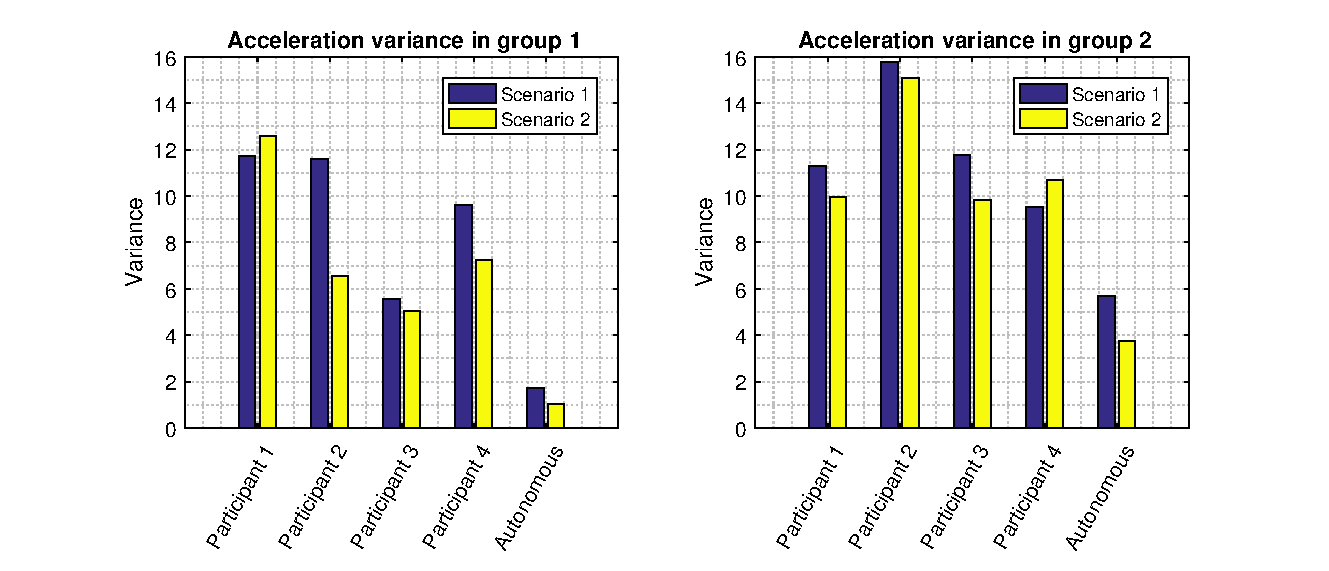
\includegraphics[width=1\linewidth]{materials/findings_and_results/acc_var.eps}}
\caption{Acceleration variance values calculated for 4 participants that took part in first and second phase and 1 autonomous car. The obvious observation is that autonomous car's acceleration varies very slightly compared to any human driver. Another observation is that variance dropped for 6 out of 8 participants when autonomous cars were introduced.}
\label{fig:acc_var}
\end{figure}


\begin{figure}[!] % Example image
\center{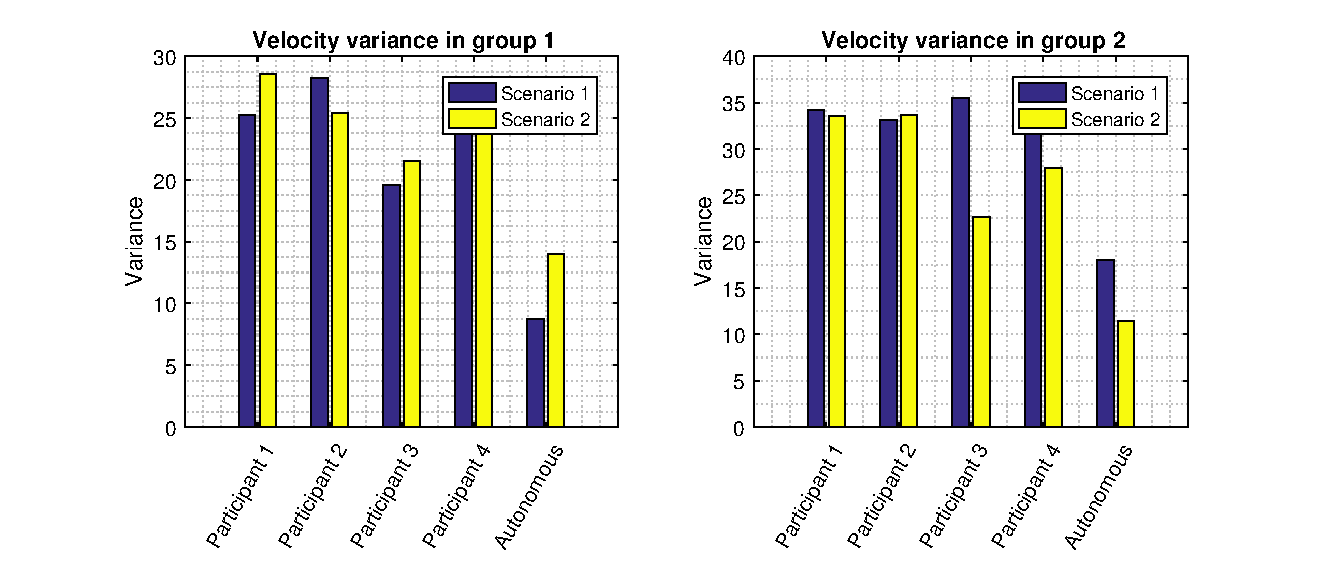
\includegraphics[width=1\linewidth]{materials/findings_and_results/vel_var.eps}}
\caption{Velocity variance values calculated for 4 participants that took part in first and second phase and 1 autonomous car. Similar to previous figure the variance values for autonomous cars were lower than those of human. However, for human drivers hardly any pattern is observable between first and second scenario.}
\label{fig:vel_var}
\end{figure} 


\paragraph{Findings}

From one point of view the impact of autonomous cars is clearly visible - average variance dropped significantly. However, if only humans are taken into consideration the differences are considerably slighter. Acceleration variance declined by 18.3\% for first group and by 5.7\% for the second group. Velocity variance in fact rose by 4.1\% for first group and declined by 12.9\% for the second group. Additionally, accounting for the fact that people's driving skill improved each round the hypothesis can only be partially confirmed:

\textbf{\textit{From the point of view of a global traffic performance, replacing a part of traditional drivers with autonomous cars smooths out traffic. It does so, because there are fewer human driver, who by nature, drive less systematically than autonomous cars. However, from the point of view of a particular driver the presence of autonomous cars does not prove to have an evident impact on driving smoothness.}}





\subsubsection{Hypothesis: Most efficient traffic could be achieved with solely autonomous vehicles}
\paragraph{}
According to \citet{litman2014autonomous} most benefits of autonomous cars will be experienced only when human drivers will completely disappear from the roads. In previous section it was shown that autonomous cars exhibit highly efficient interactions with each other. In line with these examples, very good traffic parameters should be observable for simulation involving only autonomous cars. The following hypothesis was proposed:

\textbf{\textit{For traffic consisting solely of autonomous cars parameters such as: total distance covered, acceleration variance and number of collisions should improve in comparison to traffic consisting of both types of vehicles.}}

\paragraph{Method of analysis}
In order to evaluate the hypothesis a simulation on the map used in the first and second scenario with 7 autonomous cars and no human drivers was conducted. Apart from measuring parameters mentioned in the hypothesis it was checked whether any kind of equilibrium was reached for this particular shape of the track. In addition to this, trials with different densities of vehicles were made using map from the third scenario. 




\paragraph{Findings}

A trial run on the map from the first and second scenario showed there were no collisions at all. Total distance covered by all cars was 13.4 km. For the first group this value was 11.27 km in the first scenario and 9.96 km in the second scenario. Therefore, autonomous cars travelled further even though their velocity was limited to $10\:\nicefrac{m}{s}$ which was 33\% lower than what human-driven cars were capable of. Average variance on the acceleration was 0.7850 which was 11 times smaller than the smallest value from scenario 1. Values for particular vehicles are shown on Figure~\ref{fig:acc_autonomous_only_var}. On the grounds of these finding the hypothesis can be confirmed:


For traffic consisting solely of autonomous cars parameters such as: total distance covered, acceleration variance and number of collisions should improve in comparison to traffic consisting of both types of vehicles.


\textit{\textbf{Traffic consisting only of autonomous cars will perform significantly better than traffic consisting of both types of vehicles}}


\par

As an additional topic of interest, it was investigated whether cars reach a velocity equilibrium. The results showed that indeed on track from the first scenario, the equilibrium is reached after 1.5 minute (Figure~\ref{fig:equilibrum}). However, the value of this measure can be little to none. The simulation was run on a closed track with no intersections and there was no randomization introduced at any point of the simulation apart form the initial placement of vehicles. 

%***..write more about it...

\begin{figure}[!] % Example image
\center{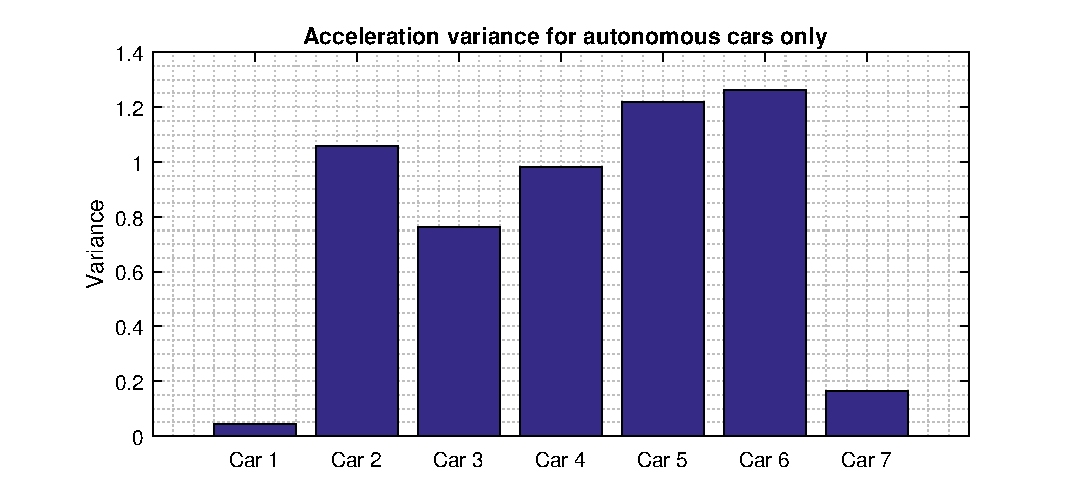
\includegraphics[width=1\linewidth]{materials/findings_and_results/acc_autonomous_only_var.eps}}
\caption{Variances of the acceleration for simulation involving only autonomous cars. The values for each car were multiple times lower than in any trial with human drivers. Additionally cars 1 and 7 travelled with even less interruption. This is probably because their initial placement allowed to reach maximum speed before other vehicles. Consequentially, they were always given higher priority at the intersection.}
\label{fig:acc_autonomous_only_var}
\end{figure} 


\begin{figure}[!] % Example image
\center{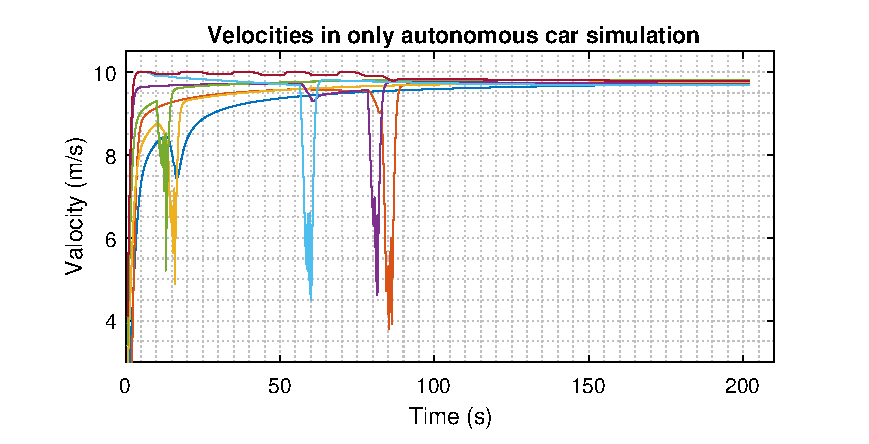
\includegraphics[width=1\linewidth]{materials/findings_and_results/equilibrum.eps}}
\caption{}
\label{fig:equilibrum}
\end{figure} 






%what is the method and why it makes sense

%- run trials with only autonomous cars. 7 cars on figure of 8 and 8 cars on scenario 3.
%Additionaly enlarge number of vehicles to maximum for figure of 8 (or scenario 3 too?)
%-find if velocity reaches some equilibrum..




%when traffic will consist solely of them.

%will be experienced only when autonomous cars
%become common and affordable


%statement of the hypothesis
%Premise: autonomous cars show much more optimized reactions between each other compared to interaction h-h or h-a





%\subsubsection{Hypothesis: Interactions were better between two human drivers rather than human and autonomous}

%***DRAFT***



%statement of the hypothesis
%Premise: autonomous car algorithm make them always give way to humna driver if the collision is anticipated. However, if the human driver will also slow down it might be possible that autonomous car will not anticipate collision any more and will start to move. This can cause another   

%\paragraph{Method of analysis}

%what is the method and why it makes sense

%- run trials with only autonomous cars. 7 cars on figure of 8 and 8 cars on scenario 3.
%Additionaly enlarge number of vehicles to maximum for figure of 8 (or scenario 3 too?)
%-find if velocity reaches some equilibrum..

%\paragraph{Findings}

%Describe you you did and what you got as a results







\newpage

\section{Conclusions and Discussion}
%METHODS!!
\paragraph{}
This section attempts to evaluate to which extent, each of the aims and objectives were met. Furthermore, the overall significance of the study is reflected upon. Ideas for future development are also provided. 

The primary objective was to conduct the experiment and so the preparation and the implementation of the experiment was at the heart of the project. In line with the original guidelines of the experiment it was possible to simultaneously connect multiple human
participants to an on-line traffic simulation.

The second objective was to engineer software that would allow to conduct the experiment. Such software was created and the previous chapters presented how it addressed all major requirements of the experiment. Nevertheless, apart from its advantages, the software had certain imperfections, such as not being able to accommodate for the originally planned number of participants (from 10 to 20).

Another task was to create a useful model of the autonomous car. The model used in the experiment derived from the well-established Intelligent Driver Model. Additional modifications performed on top of the original algorithm equipped autonomous vehicles with an ability to anticipate all kinds of collisions. The resulting model featured predictable behaviour and enabled smooth travel among other vehicles. Nevertheless, due to certain shortcomings in the design, there were situations when a self-driving vehicle was the one responsible for the collision.

The last major objective was to create a model of a car, that would be controlled by the
experiment participant. An appropriate model was developed on the basis of the dynamics
of Gipps’ car-following model.


\textbf{It is clear from the aforementioned evidence that the study successfully addressed all its objectives.} 

\par

The conclusions drawn from the research confirmed the three hypotheses which were the significant  points of this dissertation. It was proved that the autonomous revolution will bring many changes. As the results of the experiment suggest, introducing autonomous cars and in the same time reducing the number of human drivers, can help to smooth out the traffic. However, from the point of view of an individual driver the driving smoothness is not impacted significantly. Moreover, introduction of these vehicles will allow people to reevaluate their commute routine and will popularise long distance travel, as an indirect consequence. In addition to that, the total distance covered, acceleration variance and number of collisions will improve once the traffic is solely comprised of autonomous vehicles. 



These statements do not mean, that the mere introduction of a few autonomous cars will automatically imply less accidents. It is simply not possible to replace all of the human driven vehicles with autonomous ones all at once. The reasons for that are many and are not a topic of interest to this dissertation. We will have to endure a so called transition period, when autonomous cars will have to coexist with traditional vehicles. During that time the core of the most salient concern will remain unchanged. Paradoxically, humans will still be the most error prone element of the driving environment. Their often unpredictable behaviour on the road, as well as a non-satisfactory response reaction in times of danger will still be the biggest threat to road safety. Further research into the issue of coexistence is definitely needed. In my personal opinion, it should be the main focus of subsequent research. 



As it comes to the possible improvements for the experiment itself, the main issue that could be worked on is the upgrade of the software used to conduct the research. By enhancing its capabilities, more participants could take part in the project, thus making the gathered data more representative and would allow to extrapolate the findings more accurately.


 
I sincerely hope that this dissertation will propel the reader into a more extensive research of the autonomous car issue. We are facing a future in which autonomous vehicles are not a mere whim of the few, but a reality. The sooner we will be able to properly assess all the daunting questions correlated with the dilemmas this issue brings, the better. First autonomous cars are already being tested and their number will rise with every year. If we will be able to design them in a way that prevents as many accidents as possible, our roads will  become a safer environment and in consequence many lives will be saved.




%******************************************************

%end of refereing to obhectives





%\includegraphics*[100,100][300,300]{mypicture}

%\begin{figure}[H] % Example image
%\center{\includegraphics[width=0.5\linewidth]{placeholder}}
%\caption{Example image.}
%\label{fig:speciation}
%\end{figure}




%------------------------------------------------



%\begin{description} % Numbered list example

%\item[First] \hfill \\


%\item[Second] \hfill \\


%\item[Third] \hfill \\


%\end{description} 

%t

%----------------------------------------------------------------------------------------
%	CONCLUSION
%----------------------------------------------------------------------------------------



%----------------------------------------------------------------------------------------
%	BIBLIOGRAPHY
%----------------------------------------------------------------------------------------
\newpage

\bibliography{dissertation_citation_database}

%\printbibliography


%\begin{thebibliography}{99} % Bibliography - this is intentionally simple in this template

%\bibitem[Figueredo and Wolf, 2009]{Figueredo:2009dg}
%Figueredo, A.~J. and Wolf, P. S.~A. (2009).
%\newblock Assortative pairing and life history strategy - a cross-cultural
%  study.
%\newblock {\em Human Nature}, 20:317--330.
 
%\end{thebibliography}





%----------------------------------------------------------------------------------------

\end{document}